% !TEX TS-program = pdflatex
% !TEX encoding = UTF-8 Unicode

% Matthew Urffer Master Thesis
% 

%%%%%%%%%%%%%%%%%%%%%%%%%%%%%%%%%%%%%%%%%%%%%%%%%%%%%%%%%%%%%%%%%%%%%%%%%%%%%%%
% 																							         %
%					                         PREAMBLE      								%
%																										%
%%%%%%%%%%%%%%%%%%%%%%%%%%%%%%%%%%%%%%%%%%%%%%%%%%%%%%%%%%%%%%%%%%%%%%%%%%%%%%%
\documentclass[compress]{beamer}

\mode<presentation>
{
  %\usetheme{Boadilla}
  \usetheme{Frankfurt}
  \usecolortheme{crane}
  \setbeamercovered{transparent}
}

% Package Setup
\usepackage[english]{babel}
\usepackage[utf8]{inputenc}
\usepackage{times}
\usepackage[T1]{fontenc}
\usepackage{multicol}
\usepackage{array}				% Table Stuff
\usepackage{arydshln}
\usepackage{multirow}
\usepackage{rotating}
\usepackage{graphics}
\usepackage{caption}            % Caption Stuff
\captionsetup{font=scriptsize,labelfont=scriptsize}
\usepackage{amsmath}				% Math Stuff
\usepackage{listings}				% Code Example Stuff
\bibliographystyle{ieeetr}

\lstset{% General Listing Settings
	basicstyle=\tiny,
	frame=single
}


% Preamble / Frst Size
\setbeamersize{text margin left=5mm, text margin right 5mm}
\title[Matthew Urffer Master's Thesis] {Design of a Neutron Detector Capable of Replacing ${}^3$He Detectors Utilizing Thin Polymeric Films}
\subtitle{Master's Thesis Defense}
\author[] {Matthew Urffer\inst{1} }
\institute[University of Tennessee] { 
  \inst{1}%
  Department of Nuclear Engineering\\
  University of Tennessee, Knoxville, TN
}

\date[] {November 8th, 2012}
\pgfdeclareimage[height=0.5cm]{university-logo}{images/utwordmarkhorz.eps}
\logo{\pgfuseimage{university-logo}}


% Delete this, if you do not want the table of contents to pop up at
% the beginning of each subsection:
\AtBeginSection[]
{
  \begin{frame}<beamer>{}
    \frametitle{\insertsectionhead}
    \begin{multicols}{2}
  % \tableofcontents[currentsubsection,hideothersubsections,sectionstyle=show/hide,subsectionstyle=show/shaded,]
    \tableofcontents[currentsection] 
    \end{multicols}
  \end{frame}
}


% If you wish to uncover everything in a step-wise fashion, uncomment
% the following command: 
%\beamerdefaultoverlayspecification{<+->}


\begin{document}

\begin{frame}
  \titlepage
\end{frame}

\begin{frame}{Table of Contents}
  \begin{multicols}{2}
    %\tableofcontents[currentsection,pausesections]
    \tableofcontents[currentsection]
    \end{multicols}
\end{frame}


%%%%%%%%%%%%%%%%%%%%%%%%%%%%%%%%%%%%%%%%%%%%%%%%%%%%%%%%%%%%%%%%%%%%%%%%%%%%%%%
%                                                                             %
%                             START OF CONTENT                                %
%                                                                             %
%%%%%%%%%%%%%%%%%%%%%%%%%%%%%%%%%%%%%%%%%%%%%%%%%%%%%%%%%%%%%%%%%%%%%%%%%%%%%%%
% !TEX TS-program = pdflatex
% !TEX encoding = UTF-8 Unicode

% Matthew Urffer Master Thesis
% INTRODUCTORY MATERIAL 

\section{Introduction}

\subsection{Radiation Portal Monitors}

%%%%%%%%%%%%%%%%%%%%%%%%%%%%%%%%%%%%%%%%%%%%%%%%%%%%%%%%%%%%%%%%%%%%%%%%%%%%%%%
\begin{frame}{U.S. Border Traffic}
\begin{columns}[onlytextwidth]
\begin{column} {0.45\textwidth}
 
  \begin{itemize}
  \item Every day 932,456 people cross into the U.S. \cite{cpb_typical_2012}
    \begin{itemize}
    	\item 259,191 by air
	\item 48,073 by sea
	\item 621,874 by land
    \end{itemize}
  \item 64,483 truck, rail and sea containers \cite{cpb_typical_2012}
 \item 253,821 privately-owned vehicles \cite{cpb_typical_2012}
  \end{itemize}
\end{column}
\begin{column}{0.45\textwidth}
\centering
\begin{figure}
		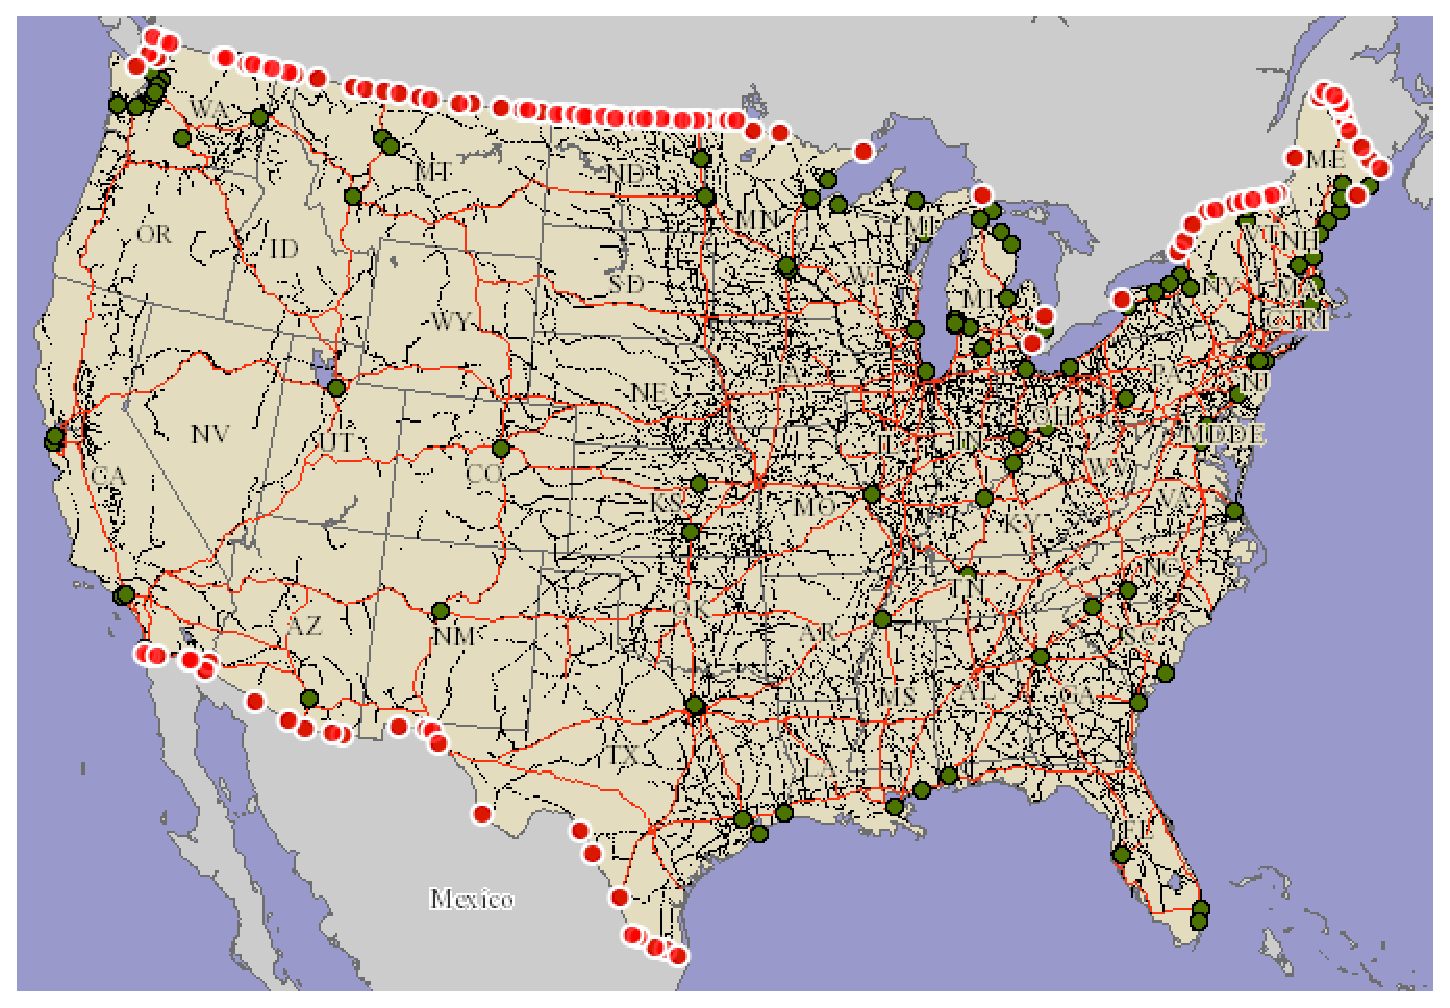
\includegraphics[width=\textwidth]{images/PortalEntryMap.eps}
		\label{fig:PortalEntryMap}
	\caption{Portal Entry Points into the U.S.}
\end{figure}
\end{column}
\end{columns}
\end{frame}

%%%%%%%%%%%%%%%%%%%%%%%%%%%%%%%%%%%%%%%%%%%%%%%%%%%%%%%%%%%%%%%%%%%%%%%%%%%%%%%
\begin{frame}{Radiation Portal Monitors}
\begin{columns}[onlytextwidth]
	\begin{column} {0.45\textwidth}
  	\begin{itemize}
  		\item Radiation portal monitors (RPMs) are passive radiation detectors
  		\item {
  			 RPMs are currently   ${}^3$He based detectors
  			\center
    		${}^3He +n \to p +{}^3H$
    	}
  		\item 
  			Shortage of ${}^3$He, so alternatives are being explored
  		\end{itemize}
	\end{column}
	\begin{column}{0.5\textwidth}
		\centering
		\begin{figure}
			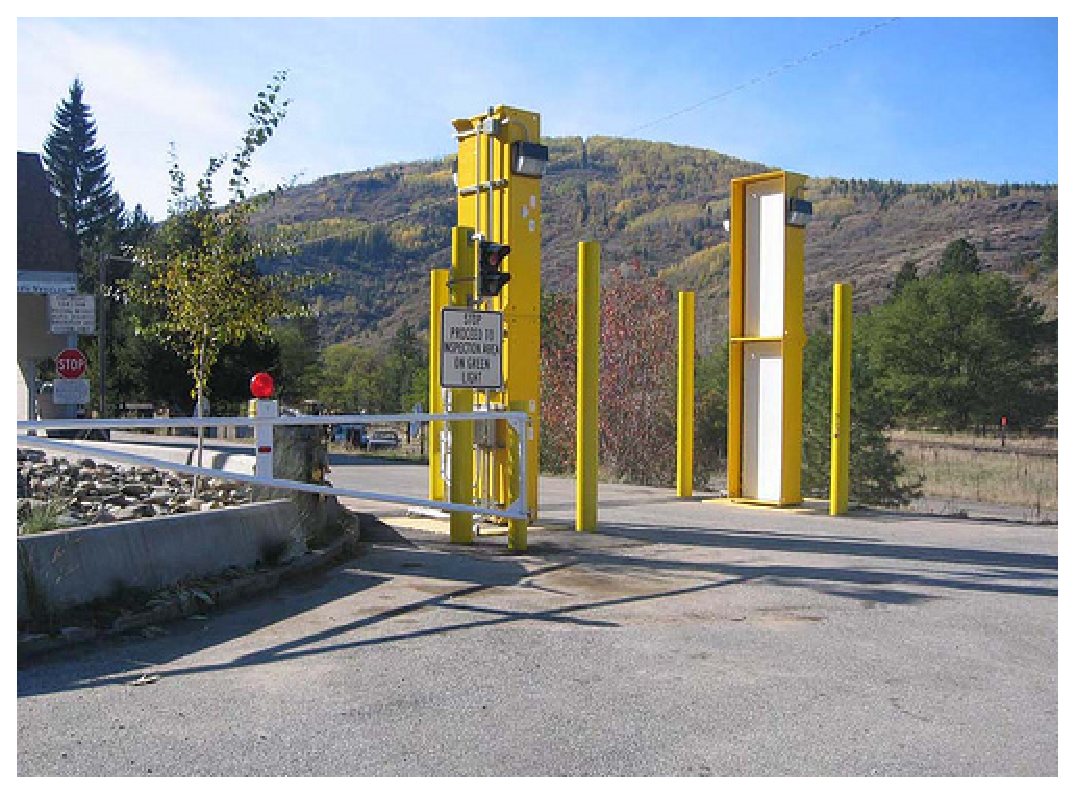
\includegraphics[width=\textwidth]{images/RPM8_Installed.eps}
			\label{fig:RPM8Installed}
			\caption{Installed RPM}
			\end{figure}
	\end{column}
\end{columns}
\end{frame}


%%%%%%%%%%%%%%%%%%%%%%%%%%%%%%%%%%%%%%%%%%%%%%%%%%%%%%%%%%%%%%%%%%%%%%%%%%%%%%%
\begin{frame}{Neutron Adsorption Interactions}
\begin{itemize}
	\item Desired reaction properties
	\begin{itemize}
		\item High probability of occurrence
		\item Ease of detecting reaction products
		\item Reaction products have a low pulse height deficit
	\end{itemize}
\end{itemize}
\begin{table}
	\tiny
	\begin{tabular}{ c | c c c} 
		Reaction                           & Q-Value (MeV) & Thermal Cross Section & Application \\
		\hline
		\hline
		${}^3He + n \to p +{}^3H$          & 0.756     & 5,330 & Proportional counter gas \\
		${}^6Li + n \to {}^3H + \alpha$    & 4.78      & 940 & Lithium glass scintillators \\
		${}^{10}B + n \to \alpha + {}^7Li$ & 2.31      & 3,840 & Plastic scintillators \\
		${}^{157}Gd + n \to \gamma$        &various    & 259,000 & various \\
	\end{tabular}
\end{table}
\end{frame}

%%%%%%%%%%%%%%%%%%%%%%%%%%%%%%%%%%%%%%%%%%%%%%%%%%%%%%%%%%%%%%%%%%%%%%%%%%%%%%%
\begin{frame}{Energy Deposition (Charged Particle)}
Products of ${}^6$Li neutron interaction are triton and alpha:
\begin{columns}[onlytextwidth]
\begin{column}{0.45\textwidth}
\begin{itemize}
	\small
	\item Alpha Energy: 2.05 MeV
	\item Triton Energy: 2.73 MeV
\end{itemize}
Alpha and tritons tend to deposit all of their energy in a small region
\end{column}
\begin{column}{0.45\textwidth}
	\begin{figure}
	\includegraphics[width=\textwidth]{images/PStarAStarRange.eps}
	\caption{Alpha and Triton Range (CSDA) \protect \cite{berger_estar_2005}}
	\label{fig:PStarAStarRange}
	\end{figure}
\end{column}
\end{columns}
\end{frame}

\subsection{Detector Requirements}
%%%%%%%%%%%%%%%%%%%%%%%%%%%%%%%%%%%%%%%%%%%%%%%%%%%%%%%%%%%%%%%%%%%%%%%%%%%%%%%
\begin{frame}{Detector Requirements}
DHS / DNDO (along with PNNL) has determined a set of objectives that replacement technologies should meet:
\begin{table}
	\tiny
	\begin{tabular}{c c }
	Parameter & Specification \\
	\hline
	\hline
	Absolute neutron detection efficiency & 2.5 cps/ng of ${}^{252}Cf$ (in specified test configuration) \\
	Intrinsic gamma-neutron detection efficiency & $ \epsilon_{int,\gamma}\leq 10^{-6}$ \\
	Gamma absolute rejection ratio for neutrons (GARRn) & $ 0.9 \leq \text{ GARRn }\leq$ 1.1 at 10 mR/h exposure \\
	Cost &  \$ 30,000 per system \\
	\hline
	\end{tabular}
\end{table}
\end{frame}

%%%%%%%%%%%%%%%%%%%%%%%%%%%%%%%%%%%%%%%%%%%%%%%%%%%%%%%%%%%%%%%%%%%%%%%%%%%%%%%
\begin{frame}{Absolute Neutron Efficiency}
\newtheorem{thm1}{Absolute Neutron Efficiency}
\begin{thm1}<1->
$$\epsilon_{abs} = \frac{\text{Counts}}{\text{Quanta Radiation Emitted}}\; \; \protect \cite{knoll_radiation_2009} $$
Constraint:
$$\epsilon_{abs} \geq 2.5\; \text{cps per ng}\; {}^{252}\text{Cf}$$
\end{thm1}
Test configuration is defined to be 1 ng ${}^{252}$Cf surrounded by 0.5 cm of lead and 2.5 cm of HDPE, with the detector midpoint 2 m from the source \cite{kouzes_alternative_2010}
\end{frame}


%%%%%%%%%%%%%%%%%%%%%%%%%%%%%%%%%%%%%%%%%%%%%%%%%%%%%%%%%%%%%%%%%%%%%%%%%%%%%%%
\begin{frame}{Intrinsic Gamma-Neutron Detection Efficiency}
\newtheorem{thm2}{Intrinsic Gamma-Neutron Detection Efficiency}
\begin{thm2}<1->
$$\epsilon_{int,n \gamma} = \frac{\text{Counts}}{\text{Quanta Radiation Crossing Detector}} \; \protect \cite{kouzes_alternative_2010} $$
Constraint:
$$ \epsilon_{int,n \gamma} \leq 10^{-6} $$
\end{thm2}
\begin{itemize}
	\item Counts over quanta crossing the detector
	\item Measured from a source that produces a 10 mR/hr field
\end{itemize}
\end{frame}

%%%%%%%%%%%%%%%%%%%%%%%%%%%%%%%%%%%%%%%%%%%%%%%%%%%%%%%%%%%%%%%%%%%%%%%%%%%%%%%
\begin{frame}{Gamma Absolute Rejection Ratio}
\newtheorem{thm3}{GARRn}
\begin{thm3}<1->
$$ GARRn = \frac{\epsilon_{\gamma,abs}}{\epsilon_{n,abs}} \; \protect \cite{kouzes_alternative_2010} $$
Constraint:
$$ 0.9 \leq GARRn \leq 1.1 $$
\end{thm3}
The detector's performance should change by no more than 10\% in a strong gamma field
\begin{itemize}
	\item GARRn is measured by exposing the detector to a 10 mR/hr gamma field while exposed to neutron source
	\item Count rate is measured when the gamma source is no longer present
	\item Difference determines the GARRn
\end{itemize}
\end{frame}

%%%%%%%%%%%%%%%%%%%%%%%%%%%%%%%%%%%%%%%%%%%%%%%%%%%%%%%%%%%%%%%%%%%%%%%%%%%%%%%
%                                                                             %
%                                PREVIOUS WORK                                %
%                                                                             %
%%%%%%%%%%%%%%%%%%%%%%%%%%%%%%%%%%%%%%%%%%%%%%%%%%%%%%%%%%%%%%%%%%%%%%%%%%%%%%%
\subsection{Previous Work}

%%%%%%%%%%%%%%%%%%%%%%%%%%%%%%%%%%%%%%%%%%%%%%%%%%%%%%%%%%%%%%%%%%%%%%%%%%%%%%%
\begin{frame}{Replacement Technologies (Boron)}
\begin{columns}[onlytextwidth]
\begin{column}{0.45\textwidth}
\begin{itemize}
	\small
	\item Boron Straw Tubes (Proportional Technology) \cite{kouzes_boron-lined_2012}
	\begin{itemize}
		\tiny
		\item Count rate meets requirements
		\item Gamma rejection is estimated to be $4x10^{-9}$
		\item GARRn within desired range
	\end{itemize}
	\small
	\item Boron Triflouride Gas Detectors (LND) \cite{kouzes_bf3_2009}
	\begin{itemize}
		\tiny
        \item Two tubes are marginally able to replace one ${}^3$He tube
		\item BF${}_3$ Tubes require 2200V to operate than ${}^3$He tubes (1000 V)
		\item BF${}_3$ Tubes require less pressure than ${}^3$He tubes
	\end{itemize}
\end{itemize}
\end{column}
\begin{column}{0.45\textwidth}
	\begin{figure}
	\centering
		\includegraphics[height=0.25\textheight]{images/B10StrawFibers.eps}
		\caption{ ${}^{10}$B Straw Fibers}
		\label{fig:B10StrawFibers}
		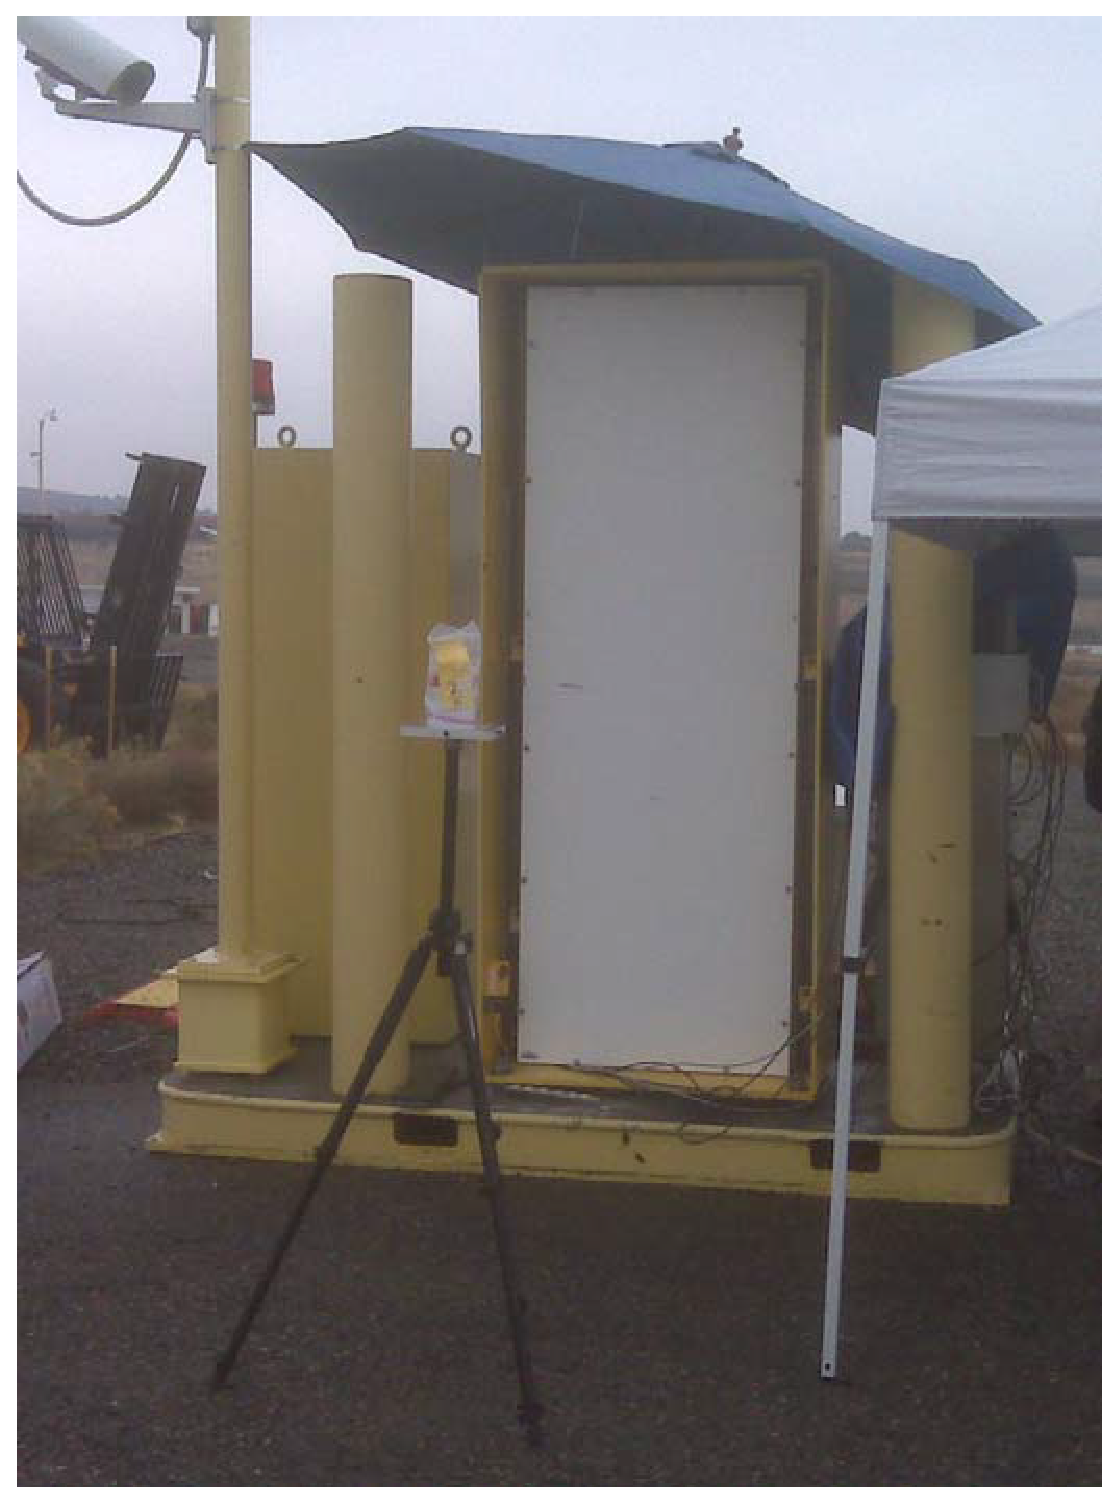
\includegraphics[height=0.25\textheight]{images/BF3Test.eps}
		\caption{PNNL test of BF${}_3$ Detector}
		\label{fig:BF3PNNLTest}
	\end{figure}
\end{column}
\end{columns}
\end{frame}

%%%%%%%%%%%%%%%%%%%%%%%%%%%%%%%%%%%%%%%%%%%%%%%%%%%%%%%%%%%%%%%%%%%%%%%%%%%%%%%
\begin{frame}{Replacement Technologies (Lithium)}
\begin{columns}[onlytextwidth]
\begin{column}{0.45\textwidth}
\begin{itemize}
	\small
	\item LiF:ZnS coated Paddles (IAT) \cite{kouzes_lithium_2010}
	\begin{itemize}
		\item Did not fulfill the neutron count rate
		\item Adequate gamma ray rejection
		\item Passed the GARRn
	\end{itemize}
	\small
	\item NucSafe Glass Fibers\cite{kouzes_alternative_2010}
	\begin{itemize}
		\item Tested with a scale model, 1.72 cps
		\item Three filter levels for GARRn
		\begin{itemize}
			\tiny
			\item Conservative filter passed GARRn, failed count rate
			\item Other filters failed GARRn
		\end{itemize}
	\end{itemize}
\end{itemize}
\end{column}
\begin{column}{0.45\textwidth}
	\begin{figure}
		\includegraphics[height=0.25\textheight]{images/LiFZnSPaddle.eps}
		\caption{${}^6$LiF:ZnS Paddle}
		\label{fig:LifZnSPaddle}
		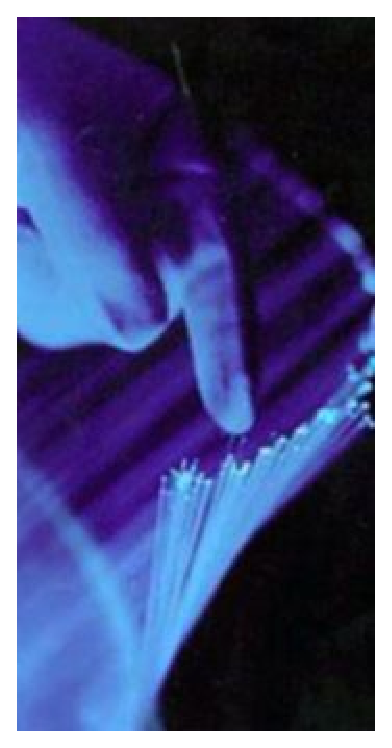
\includegraphics[height=0.25\textheight]{images/NucSafeFibers.eps}
		\caption{NucSafe Fibers}
		\label{fig:NucSafeFibers}
	\end{figure}
\end{column}
\end{columns}
\end{frame}

% !TEX TS-program = pdflatex
% !TEX encoding = UTF-8 Unicode

% Matthew Urffer Master Thesis
% 
% Methods
%
\section{Spectra Methods}

%%%%%%%%%%%%%%%%%%%%%%%%%%%%%%%%%%%%%%%%%%%%%%%%%%%%%%%%%%%%%%%%%%%%%%%%%%%%%%%
%                                                                             %
%                                   FACILITIES                                %
%                                                                             %
%%%%%%%%%%%%%%%%%%%%%%%%%%%%%%%%%%%%%%%%%%%%%%%%%%%%%%%%%%%%%%%%%%%%%%%%%%%%%%%

\subsection{Facilities}
%%%%%%%%%%%%%%%%%%%%%%%%%%%%%%%%%%%%%%%%%%%%%%%%%%%%%%%%%%%%%%%%%%%%%%%%%%%%%%%
\begin{frame}{Button Sources}
	\centering
	Alpha Sources
	\begin{table}[h]
		\tiny
		\begin{tabular}{c | c c}
		Source & Half-Life & Energy (MeV) \\
		\hline
		\hline
		${}^{232}$Th & $1.4\times10^{10}$ yr & 4.012 \\
		${}^{240}$Pu & $6.5\times10^{3}$ yr & 5.17 (76\%) 5.12 (24\%) \\
		${}^{241}$Am & 433 yr & 5.48 (85\%) 5.44 (12\%) \\
		${}^{239}$Pu, ${}^{241}$Am, ${}^{244}$Cm  & various & various \\
		\hline
		\end{tabular}
	\end{table}
	Beta Sources
	\begin{table}[h]
		\tiny
		\begin{tabular}{c | c c}
		Source & Half-Life & Endpoint Energy (MeV)\\
		\hline
		\hline
		${}^{14}$C &  5,730 yr & 0.156 \\
		${}^{36}$Cl & $3.08\times10^{5}$ yr & 0.714 \\
		${}^{36}$Ni &  92 yr & 0.067 \\
		${}^{99}$Tc & $2.12\times10^{5}$ yr & 0.292 \\
		\hline
		\end{tabular}
	\end{table}
\end{frame}

%%%%%%%%%%%%%%%%%%%%%%%%%%%%%%%%%%%%%%%%%%%%%%%%%%%%%%%%%%%%%%%%%%%%%%%%%%%%%%%
\begin{frame}{Gamma Irridiator}
\begin{columns}[onlytextwidth]
\begin{column}{0.45\textwidth}
	\begin{itemize}
		\item Desire a 10 mR/hr Gamma Field
		\item Solution is 1 100 $\mu$Ci ${}^{60}$Co source
		\item Shielded by lead
	\end{itemize}
\end{column}
\begin{column}{0.45\textwidth}
	\centering
	\begin{figure}
		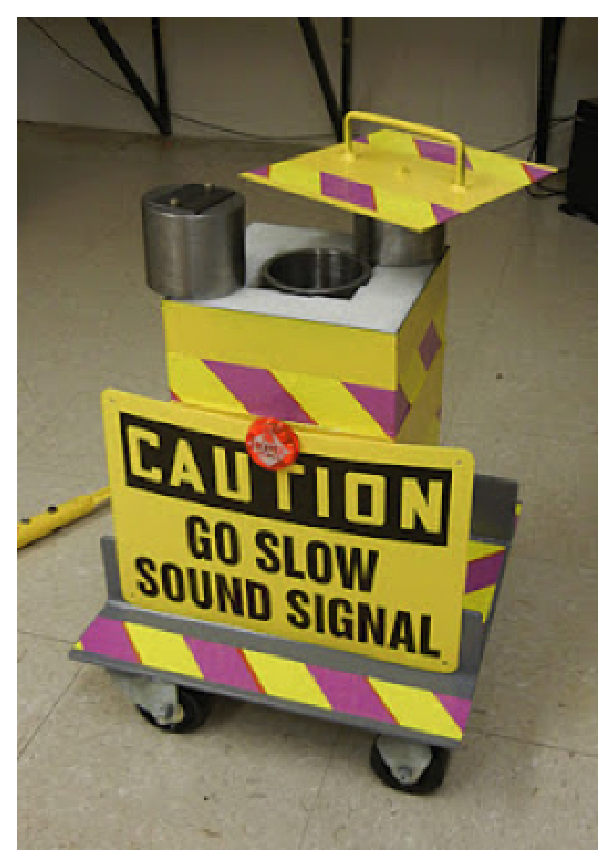
\includegraphics[width=0.8\textwidth]{images/GammaIrridiator.eps}
		\label{fig:GammaIrridiator}
		\caption{Gamma Irridiator}
	\end{figure}
\end{column}
\end{columns}
\end{frame}

%%%%%%%%%%%%%%%%%%%%%%%%%%%%%%%%%%%%%%%%%%%%%%%%%%%%%%%%%%%%%%%%%%%%%%%%%%%%%%%
\begin{frame}{Neutron Irridiator}
\begin{columns}[onlytextwidth]
\begin{column}{0.45\textwidth}
	\small
	\begin{itemize}
		\item Source is 0.59 $\mu$g ${}^{252}$Cf
		\item Encased in HDPE Box
		\item Two detector wells
		\begin{itemize}
			\tiny
			\item Lead Well
			\item Cadmium Well
		\end{itemize}
	\end{itemize}
\end{column}
\begin{column}{0.45\textwidth}
	\begin{figure}
		\centering
		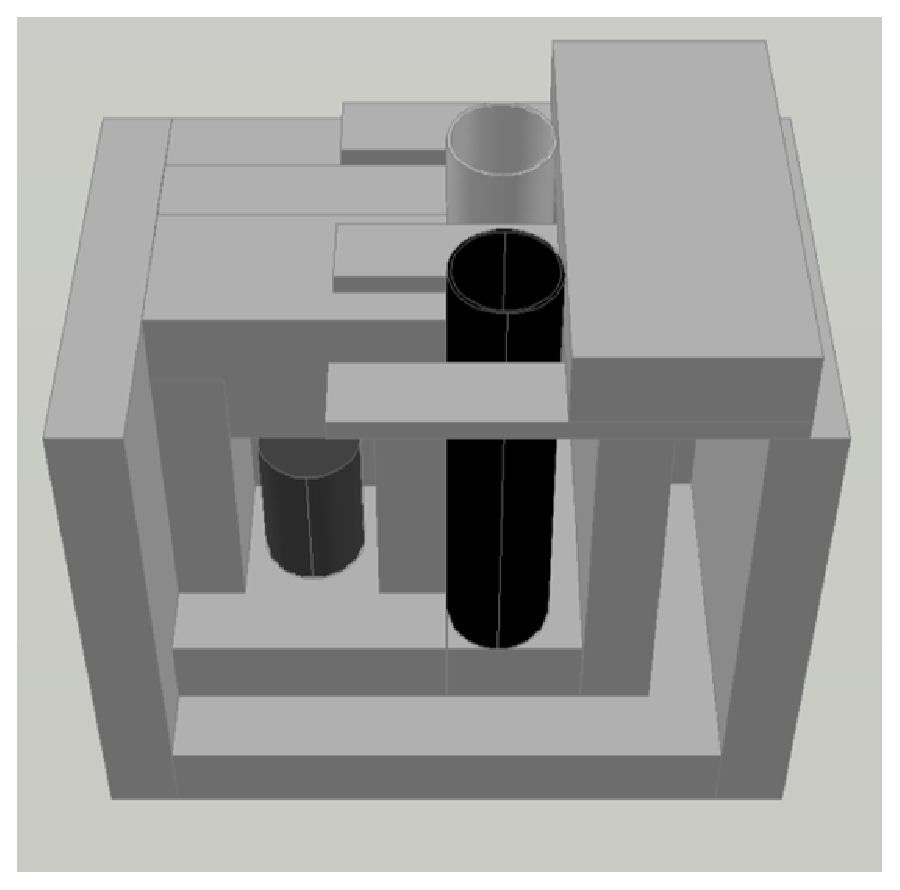
\includegraphics[height=0.25\textheight]{images/NeutronIrridiator_CAD.eps}
		\caption{CAD Rendering of Neutron Irridiator}
		\label{fig:NeutronIrridiatorCAD}
		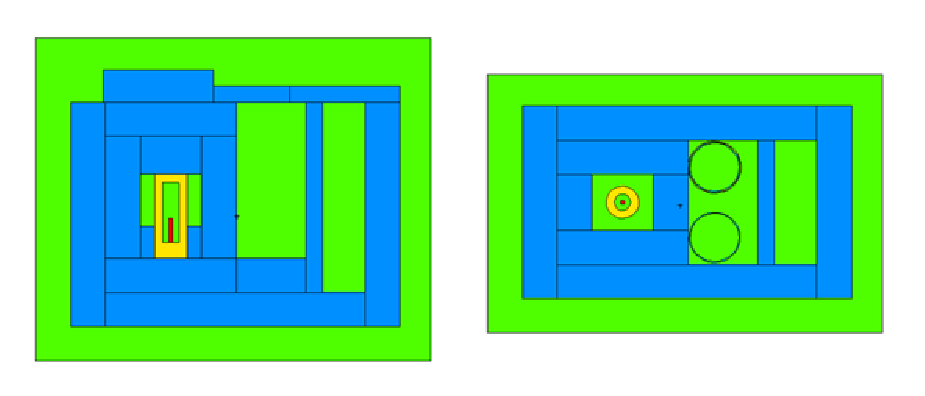
\includegraphics[height=0.25\textheight]{images/NeutronIrridiator_MCNP.eps}
		\caption{MCNPX Rendering of Neutron Irridiator}
		\label{fig:NeutronIrridiatorMNCPX}
	\end{figure}
\end{column}
\end{columns}
\end{frame}

%%%%%%%%%%%%%%%%%%%%%%%%%%%%%%%%%%%%%%%%%%%%%%%%%%%%%%%%%%%%%%%%%%%%%%%%%%%%%%%
\begin{frame}{Neutron Irridiator (Spectra)}
\begin{columns}[onlytextwidth]
\begin{column}{0.45\textwidth}
	\begin{itemize}
		\small
		\item Lead Well
		\begin{itemize}
			\tiny
			\item Neutrons of all energies
			\item Lead to match photon attenuation of cadmium
		\end{itemize}
		\small
		\item Cadmium Well
		\begin{itemize}
			\tiny
			\item Cadmium cutoff is about 0.5 eV
			\item Well response is to fast neutrons
			\item Shielding of photons from cadmium
		\end{itemize}
		\small 
		\item Subtraction is preformed between the two response to extract the response from thermal neutrons
	\end{itemize}
\end{column}
\begin{column}{0.45\textwidth}
	\begin{figure}
		\centering
		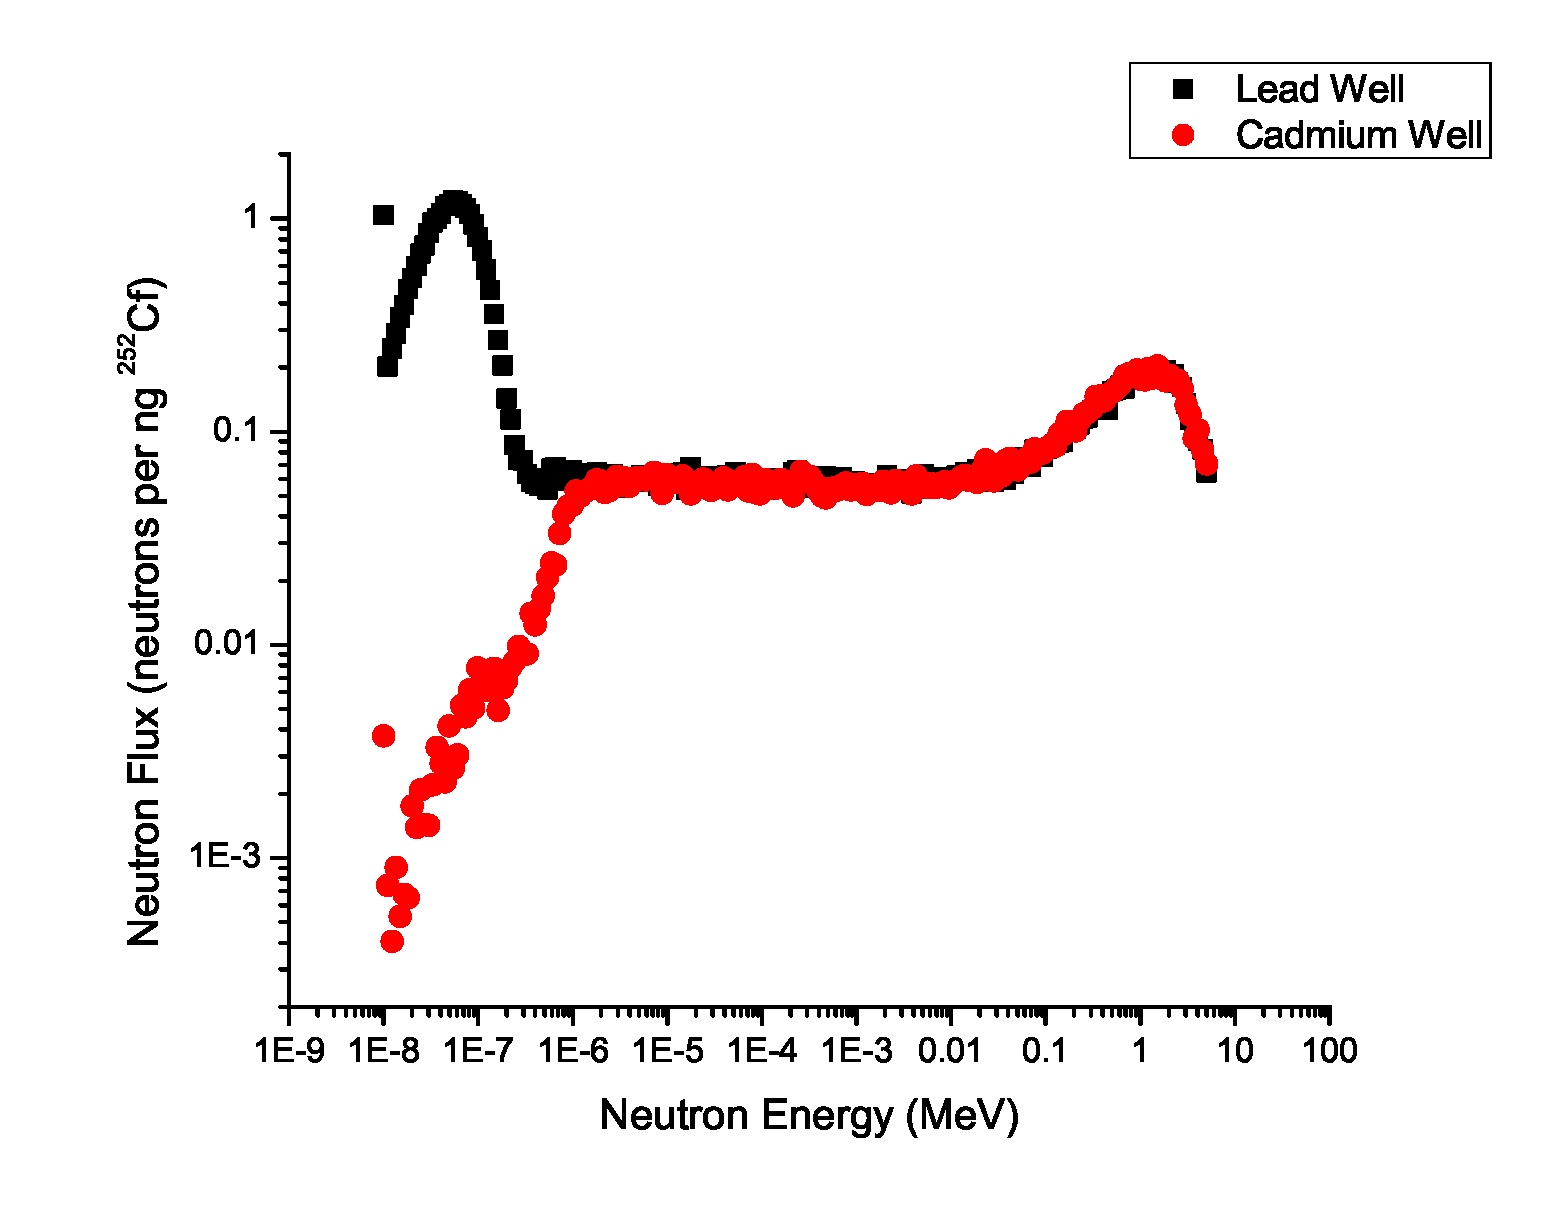
\includegraphics[height=\textwidth]{images/Graph19N.eps}
		\caption{Simulated Lead and Cadmium Well Spectra}
		\label{fig:SimPbCdSpectra}
	\end{figure}
\end{column}
\end{columns}
\end{frame}
%%%%%%%%%%%%%%%%%%%%%%%%%%%%%%%%%%%%%%%%%%%%%%%%%%%%%%%%%%%%%%%%%%%%%%%%%%%%%%%
\begin{frame}{Spectra Electronics}
\begin{columns}[onlytextwidth]
\begin{column}{0.45\textwidth}
	\small 
	Measurement Protocol
	\begin{itemize}
		\tiny
		\item Verify instrument gains are stable
		\begin{itemize}
			\tiny
			\item GS20 (${}^6$Li glass) is used as the standard
			\item Set voltage and coarse gain, adjust fine gain
		\end{itemize}
		\tiny
		\item Obtain a spectra from an alpha (${}^{241}$Am) 
		\item Obtain a spectra from a beta (${}^{36}$Cl)
		\item Obtain a lead well neutron spectra
		\item Obtain a cadmium well neutron spectra
		\item Obtain a gamma irridiator spectra
	\end{itemize}
\end{column}
\begin{column}{0.45\textwidth}
	\begin{figure}
		\centering
		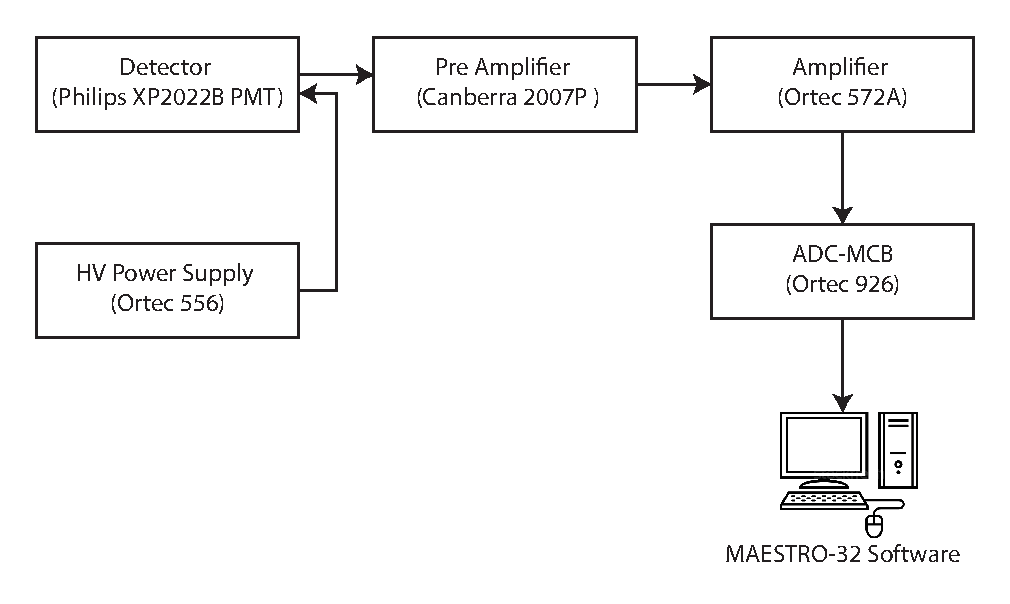
\includegraphics[height=0.5\textwidth]{images/ElectronicsSpectra.eps}
		\caption{Electronic Setup for Spectra}
		\label{fig:ElectronicsSpectra}
	\end{figure}
\end{column}
\end{columns}
\end{frame}
%%%%%%%%%%%%%%%%%%%%%%%%%%%%%%%%%%%%%%%%%%%%%%%%%%%%%%%%%%%%%%%%%%%%%%%%%%%%%%%
%                                                                             %
%                             ANALYSIS METHDOS                                %
%                                                                             %
%%%%%%%%%%%%%%%%%%%%%%%%%%%%%%%%%%%%%%%%%%%%%%%%%%%%%%%%%%%%%%%%%%%%%%%%%%%%%%%
\subsection{Analysis Methods}
%%%%%%%%%%%%%%%%%%%%%%%%%%%%%%%%%%%%%%%%%%%%%%%%%%%%%%%%%%%%%%%%%%%%%%%%%%%%%%%
\begin{frame}{Spectra Average}
	\begin{itemize}
		\item Thin films do not have clearly define features
		\item Spectra averages defined to create a feature
	\end{itemize}
	\newtheorem{thm4}{Spectra Average}
	\begin{thm4}<1->
		$$<\mu> = \frac{\int_{0}^{\infty}x f(x)dx}{\int_{0}^{\infty}f(x)dx} $$
		where:
		\begin{itemize}
			\tiny
			\item $<\mu>$ is the average of the spectra
			\item $f(x)$ is the spectra
			\item $x$ is a channel number
		\end{itemize}
	\end{thm4}
\end{frame}
%%%%%%%%%%%%%%%%%%%%%%%%%%%%%%%%%%%%%%%%%%%%%%%%%%%%%%%%%%%%%%%%%%%%%%%%%%%%%%%
\begin{frame}{Pulse Height Deficit}
	\newtheorem{thm5}{Pulse Height Deficit}
	\begin{thm5}<1->
	\tiny
	$$ PHD_{GS20} = \frac{\dfrac{n_{peak}}{4.78\;\text{MeV}}}{\dfrac{CE_\gamma}{1.038\;\text{MeV}}} $$
		where:
		\begin{itemize}
			\tiny
			\item $PHD_{GS20}$ is the pulse height deficit for GS20
			\item $n_{peak}$ is the location of the peak in the neutron spectra
			\item $CE_\gamma$ is the Compton Edge of the Gamma Spectra
		\end{itemize}
	\end{thm5}
	\newtheorem{thm6}{Pulse Height Deficit (Sample)}
	\begin{thm6}<1->
	\tiny
	$$ PHD_{Sample} = PHD_{GS20} \frac{<n>_{sample}}{<n>_{GS20}} $$
		where:
		\begin{itemize}
			\tiny
			\item $PHD_{GS20}$ is the pulse height deficit for GS20
			\item $<n>_{sample}$ is the average of the sample's neutron spectra
			\item $<n>_{GS20}$ is the average of GS20's neutron spectra
		\end{itemize}
	\end{thm6}
\end{frame}
%%%%%%%%%%%%%%%%%%%%%%%%%%%%%%%%%%%%%%%%%%%%%%%%%%%%%%%%%%%%%%%%%%%%%%%%%%%%%%%
\begin{frame}{Light Yield}
	\newtheorem{thm7}{Light Yield}
	\begin{thm7}<1->
	\tiny
	$$ LY_{n} = 3,800 \frac{\text{Photons}}{\text{MeV}}\frac{<n>_{sample}}{<n>_{GS20}} $$
	$$ LY_{\beta} = 3,800 \frac{\text{Photons}}{\text{MeV}}\frac{<\beta>_{sample}}{<\beta>_{GS20}} $$
	$$ LY_{\gamma} = 3,800 \frac{\text{Photons}}{\text{MeV}}\frac{<\gamma>_{sample}}{<\gamma>_{GS20}} $$
		where:
		\begin{itemize}
			\tiny
			\item $<n>_{sample}$ is the average of the sample's neutron spectra
			\item $<n>_{GS20}$ is the average of GS20's neutron spectra
			\item $<\beta>_{sample}$ is the average of the sample's beta (${}^{36}$Cl) spectra
			\item $<\beta>_{GS20}$ is the average of GS20's bet (${}^{36}$Cl) spectra
			\item $<\gamma>_{sample}$ is the average of the sample's gamma (${}^{60}$Co) spectra
			\item $<\gamma>_{GS20}$ is the average of GS20's gamma (${}^{60}$Co) spectra
		\end{itemize}
	\end{thm7}
\end{frame}
%%%%%%%%%%%%%%%%%%%%%%%%%%%%%%%%%%%%%%%%%%%%%%%%%%%%%%%%%%%%%%%%%%%%%%%%%%%%%%%
\begin{frame}
	\newtheorem{thm8}{Gamma Intrinsic Efficiency}
	\begin{thm8}<1->
		$$ \epsilon_{int,\gamma} = \frac{\int_{MLLD}^{\infty}{f(x)dx}}{\text{Particles Incident}} $$
	where:
	\begin{itemize}
		\tiny
		\item $MLLD$ is the mathematical lower level discriminator
		\item $f(x)$ is the spectra
		\item $\text{Particles Incident}$ is the number of incident particles
	\end{itemize}
	\end{thm8}
	\newtheorem{rmk1}{Mathematical Lower Level Discriminator}
	\begin{rmk1}
		\tiny
		Mathematical lower level discriminator (MLLD) is defined to be the channel at which $\epsilon_{int,\gamma} \leq 10^{-6}$
	\end{rmk1}

	\begin{itemize}
		\tiny
		\item MLLD for a film is determined from a ${}^{60}$Co measurement
		\item Source produces a 10 mR/hr field at detector surface
		\item Particles incident determined from simulation
	\end{itemize}
\end{frame}
%%%%%%%%%%%%%%%%%%%%%%%%%%%%%%%%%%%%%%%%%%%%%%%%%%%%%%%%%%%%%%%%%%%%%%%%%%%%%%%
\begin{frame}{Gamma Intrinsic Efficiency Example I}
	\begin{figure}
		\centering
		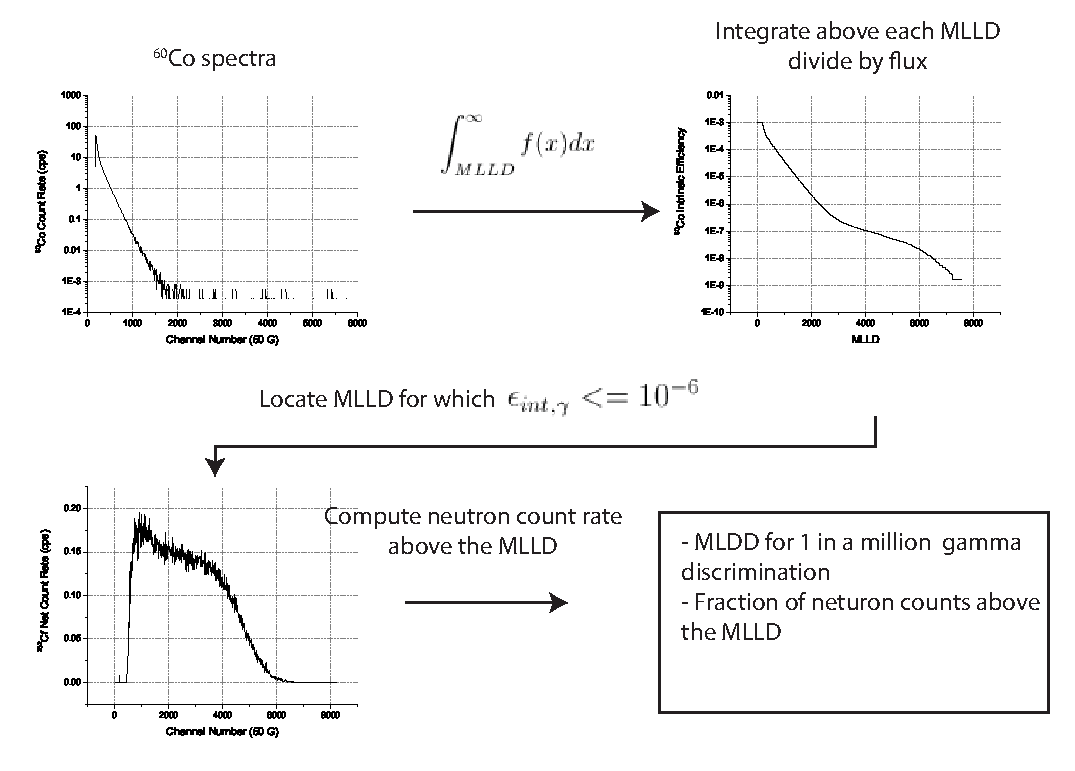
\includegraphics[height=0.5\textheight]{images/CartoonIntEffReal.eps}
		\caption{Determination of the MLLD (Example)}
		\label{fig:ElectronicsPSD}
	\end{figure}
\end{frame}
%%%%%%%%%%%%%%%%%%%%%%%%%%%%%%%%%%%%%%%%%%%%%%%%%%%%%%%%%%%%%%%%%%%%%%%%%%%%%%%
\begin{frame}{Gamma Intrinsic Efficiency Example II}
	\begin{figure}
		\centering
		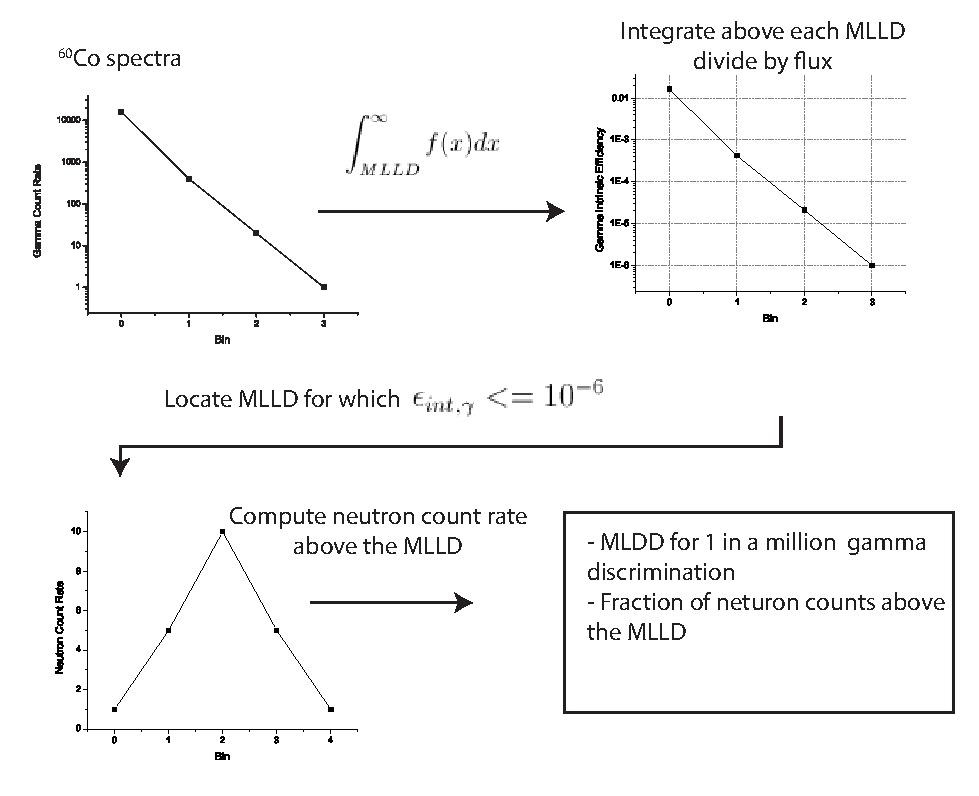
\includegraphics[height=0.5\textheight]{images/CartoonIntEffSimple.eps}
		\caption{Determination of the MLLD for a PEN film}
		\label{fig:CartoonIntEffSimple}
	\end{figure}
\end{frame}
%%%%%%%%%%%%%%%%%%%%%%%%%%%%%%%%%%%%%%%%%%%%%%%%%%%%%%%%%%%%%%%%%%%%%%%%%%%%%%%
%%%%%%%%%%%%%%%%%%%%%%%%%%%%%%%%%%%%%%%%%%%%%%%%%%%%%%%%%%%%%%%%%%%%%%%%%%%%%%%

% !TEX TS-program = pdflatex
% !TEX encoding = UTF-8 Unicode

% Matthew Urffer Master Thesis
% 
% Methods
%
\section{Simulation Methods}

%%%%%%%%%%%%%%%%%%%%%%%%%%%%%%%%%%%%%%%%%%%%%%%%%%%%%%%%%%%%%%%%%%%%%%%%%%%%%%%
%                                                                             %
%                             SIMULATION METHODS                              %
%                                                                             %
%%%%%%%%%%%%%%%%%%%%%%%%%%%%%%%%%%%%%%%%%%%%%%%%%%%%%%%%%%%%%%%%%%%%%%%%%%%%%%%
\subsection{MCNPX Simulations}
%%%%%%%%%%%%%%%%%%%%%%%%%%%%%%%%%%%%%%%%%%%%%%%%%%%%%%%%%%%%%%%%%%%%%%%%%%%%%%%
\begin{frame}{MCNPX Simulations}
	\centering
	\begin{figure}
		
\includegraphics[width=0.15\textwidth]{images/logo-mcnpx.eps}
	\end{figure}
    \small
    MCNPX is a well validated transport code \cite{pelowitz_mcnpx_2010}
\tiny
    \newtheorem{thm10}{Dose Rate Calculation}
	\begin{thm10}<1->
		$$F2 = \frac{1}{A} \int_{A}{dA}\int_{E}{dE}\int_{4\pi}{d \Omega \Re(E) \Phi(\vec{r},E,\vec{\Omega})} $$
	where:
	\begin{itemize}
		\item $\Re(E)$ is the response function
		\item $\Phi(\vec{r},E,\vec{\Omega})$ is the photon flux
	\end{itemize}
	\end{thm10}
	\newtheorem{thm11}{Interaction Rate}
	\begin{thm11}<1->
		$$Q = C \int {\Phi(E) R_m(E) dE }$$
	where:
	\begin{itemize}
		\item $C$ is a scalar normalization (density)
		\item $R_m(E)$ is the response function
		\item $\Phi(E)$ is the neutron flux
	\end{itemize}
	\end{thm11}
\end{frame}

%%%%%%%%%%%%%%%%%%%%%%%%%%%%%%%%%%%%%%%%%%%%%%%%%%%%%%%%%%%%%%%%%%%%%%%%%%%%%%%
%                                                                             %
%                             SIMULATION VALIDATION                           %
%                                                                             %
%%%%%%%%%%%%%%%%%%%%%%%%%%%%%%%%%%%%%%%%%%%%%%%%%%%%%%%%%%%%%%%%%%%%%%%%%%%%%%%
\subsection{Simulation Validation}
%%%%%%%%%%%%%%%%%%%%%%%%%%%%%%%%%%%%%%%%%%%%%%%%%%%%%%%%%%%%%%%%%%%%%%%%%%%%%%%
\begin{frame}{Gamma Dose Rate Agreement}
\small
Compared simulated to measurements prefomed by RSO
	\begin{table}[h]
		\tiny
		\begin{tabular}{c c | c c}
        \multicolumn{2}{c}{Measured} & \multicolumn{2}{c}{Simulated} \\
        Distance (cm) & Dose Rate (mRem/hr) & Distance (cm) & Dose Rate (mRem/hr) \\
		\hline
		\hline
        10.2 & 10 & 10.2 & 10.3 \\
        13 & 5.5 & 12.7 & 5.38 \\
        28 & 2 & 28 & 1.80 \\
		\end{tabular}
	\end{table}
	\centering
	\begin{figure}
		\includegraphics[height=0.5\textheight]{images/DoseRate.eps}
		\caption{Dose Rate in Detector}
	\end{figure}
\end{frame}
%%%%%%%%%%%%%%%%%%%%%%%%%%%%%%%%%%%%%%%%%%%%%%%%%%%%%%%%%%%%%%%%%%%%%%%%%%%%%%%
\begin{frame}{Neutron Simulation Agreement}
	\begin{table}[h]
	\tiny
	\begin{tabular}{m{2cm} | >{\centering\arraybackslash}m{2cm} >{\centering\arraybackslash}m{2cm} >{\centering\arraybackslash}m{2cm}}
		 & Simulated Count Rate & Observed Count Rate & Relative Error \\
		 \hline
		 \hline
		 GS20 & 424.83 $\pm$ 3.8\% & 428 & -0.7 \% \\
		 PS Film, 25 $\mu$m & 56.23 $\pm$ 1.19\% & 51 & 9.5\% \\
		 PS Film, 50 $\mu$m & 108.10 $\pm$ 1.14\% & 96 & 12.6\% \\
	\end{tabular}
	\end{table}
	\tiny
	\begin{definition}[Relative Error]
		$$\sigma = \frac{\text{Obs} -\text{ Sim}}{\text{Obs}}$$
	where:
	\begin{itemize}
		\item $\text{Obs}$ is the observed count rate
		\item $\text{Sim}$ is the simulated count rate
	\end{itemize}
	\end{definition}
\end{frame}

% !TEX TS-program = pdflatex
% !TEX encoding = UTF-8 Unicode

% Matthew Urffer Master Thesis
% 
% Pulse Shape Discrimination
%
\section{PSD Methods}

%%%%%%%%%%%%%%%%%%%%%%%%%%%%%%%%%%%%%%%%%%%%%%%%%%%%%%%%%%%%%%%%%%%%%%%%%%%%%%%
%                                                                             %
%                                    METHODS                                  %
%                                                                             %
%%%%%%%%%%%%%%%%%%%%%%%%%%%%%%%%%%%%%%%%%%%%%%%%%%%%%%%%%%%%%%%%%%%%%%%%%%%%%%%

\subsection{PSD Introduction}
%%%%%%%%%%%%%%%%%%%%%%%%%%%%%%%%%%%%%%%%%%%%%%%%%%%%%%%%%%%%%%%%%%%%%%%%%%%%%%%
\begin{frame}{Introduction to PSD}
	\begin{itemize}
		\small
		\item Determination of incident radation from pulse shape
		\item Physical basis
		\begin{itemize}
			\tiny
			\item Difference in singlet ($S_1$) and triplet ($T_1$) states \cite{zaitseva_plastic_2012}
			\item Triple states annihilate: $T_1 + T_1 \to S_0 + S_1$
			\item Product states have a longer and delayed time scale
		\end{itemize}
		\small
		\item Short range of energetic protons (neutron interactions) cause a high concentration of triplet states than from electrons from gamma
		\item Lots of methods exist \cite{ambers_hybrid_2011, gamage_comparison_2011, miller_digital_2007}
		\begin{itemize}
			\tiny
			\item Charge Integration
			\item Pulse Gradient Analysis
			\item Neutron-$\gamma$ Modal Analysis
			\item Pulse Shape Parameters
			\item Artifical Neural Networks
			\item and more!
		\end{itemize}
	\end{itemize}
\end{frame}
%%%%%%%%%%%%%%%%%%%%%%%%%%%%%%%%%%%%%%%%%%%%%%%%%%%%%%%%%%%%%%%%%%%%%%%%%%%%%%%
\begin{frame}{Pulse Height Electronics}
	\begin{itemize}
		\small
		\item Pulse traces are recorded either from an oscilloscope or from fast digitilizer
		\item Requires fast PMT and electroncis
	\end{itemize}
	\begin{figure}
		\centering
		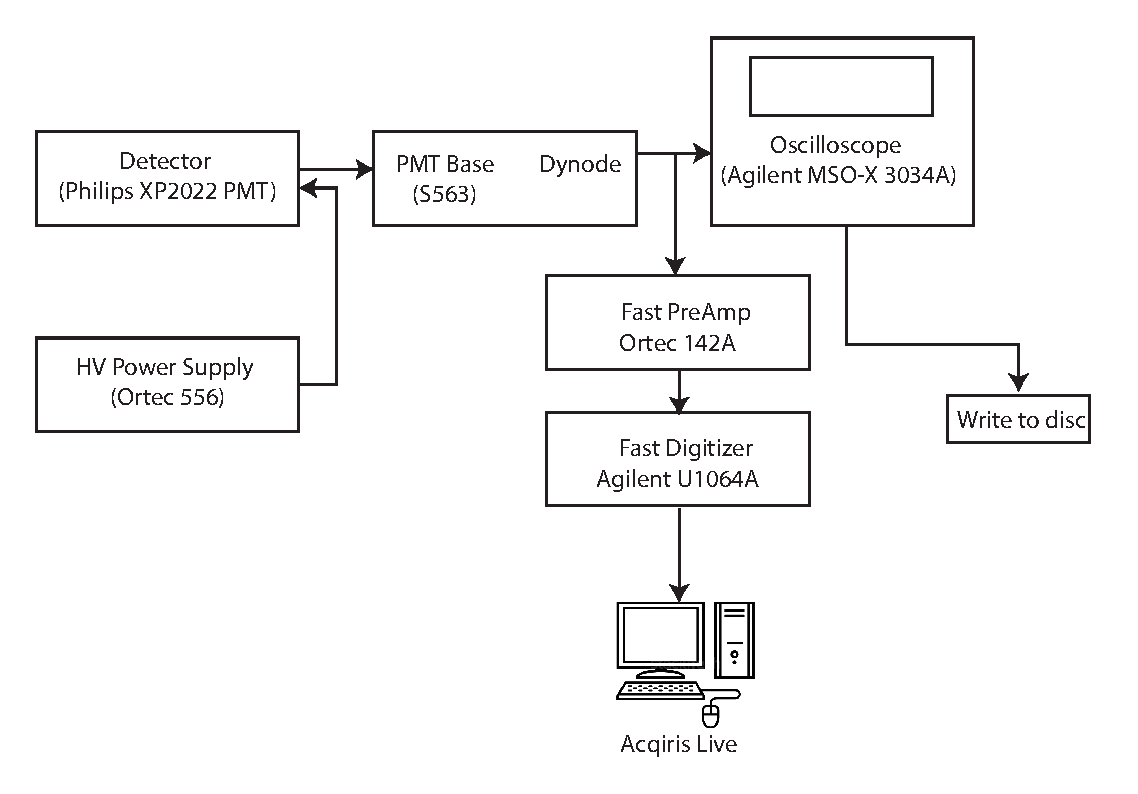
\includegraphics[height=0.5\textheight]{images/ElectronicsPSD.eps}
		\caption{Electronic Setup for Pulse Shape}
		\label{fig:ElectronicsPSD}
	\end{figure}
\end{frame}
%%%%%%%%%%%%%%%%%%%%%%%%%%%%%%%%%%%%%%%%%%%%%%%%%%%%%%%%%%%%%%%%%%%%%%%%%%%%%%%
\begin{frame}{PSD Methods}
\begin{columns}[onlytextwidth]
\begin{column}{0.45\textwidth}
	Alpha are used as surrogate neutrons
	\newtheorem{thm9}{Charge Ratio Method}
	\begin{thm9}<1->
		$$ R_C = \frac{\int_{X_0}^{\infty}{f(x)dx}}{\int_{0}^{\infty}{f(x)dx}} $$
	where:
	\begin{itemize}
		\tiny
		\item $R_C$ is the charge ratio
		\item $f(x)$ is the spectra
		\item $\int_{X_0}^{\infty}{f(x)dx}$ slow charge
		\item $\int_{0}^{\infty}{f(x)dx}$ fast charge
	\end{itemize}
	\end{thm9}
\end{column}
\begin{column}{0.45\textwidth}
	\begin{figure}
		\centering
		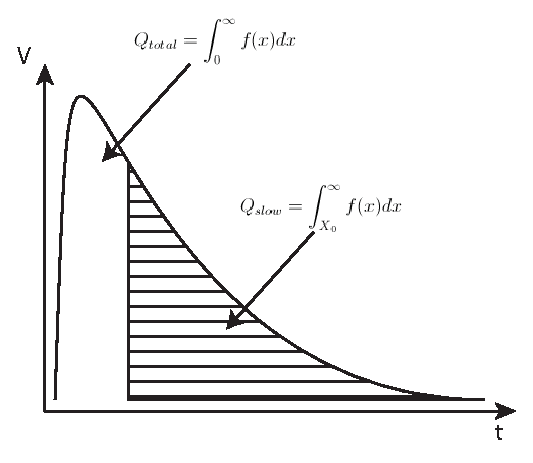
\includegraphics[height=0.5\textwidth]{images/PSD_Spectra.eps}
		\caption{Charge Ratio Method}
		\label{fig:PSD_ChargeRatio}
	\end{figure}
\end{column}
\end{columns}

	\begin{itemize}
		\tiny
		\item MLLD for a film is determined from a ${}^{60}$Co measurement
		\item Source produces a 10 mR/hr field at detector surface
		\item Particles incident determined from simulation
	\end{itemize}
\end{frame}
%%%%%%%%%%%%%%%%%%%%%%%%%%%%%%%%%%%%%%%%%%%%%%%%%%%%%%%%%%%%%%%%%%%%%%%%%%%%%%%
\begin{frame}{ROC Curves I}
	\begin{table}[h]
	\small
	\begin{tabular}{m{1cm} | m{1.5cm}| >{\centering\arraybackslash}m{2cm} >{\centering\arraybackslash}m{2cm}}
		 & \multicolumn{3}{c}{True Class} \\
		 \hline
		 \hline
		 \multirow{3}{*}{\protect \begin{sideways} Hypothesized Class \protect \end{sideways}} & & Alpha & Gamma \\  \cline{3-4}
		 & Alpha & True Postive & False Postive (Type 1) \\ \cdashline{3-4}
		 & Gamma & False Negative (Type 2) & True Negative \\ 
	\end{tabular}
	\end{table}
	\begin{figure}
		\centering
		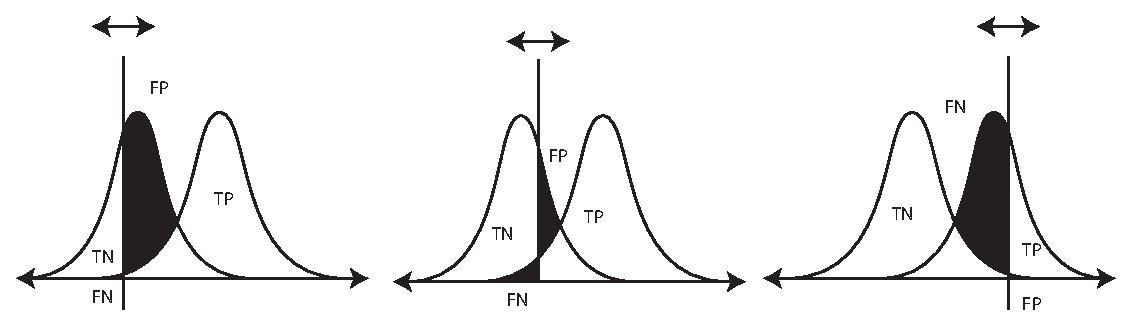
\includegraphics[width=0.75\textwidth]{images/ROC_Diagrams.eps}
		\caption{Perforamnce of a Classifier}
		\label{fig:ROCDiagrams}
	\end{figure}
\end{frame}
%%%%%%%%%%%%%%%%%%%%%%%%%%%%%%%%%%%%%%%%%%%%%%%%%%%%%%%%%%%%%%%%%%%%%%%%%%%%%%%
\begin{frame}{ROC Curves II}
	\begin{figure}
		\centering
		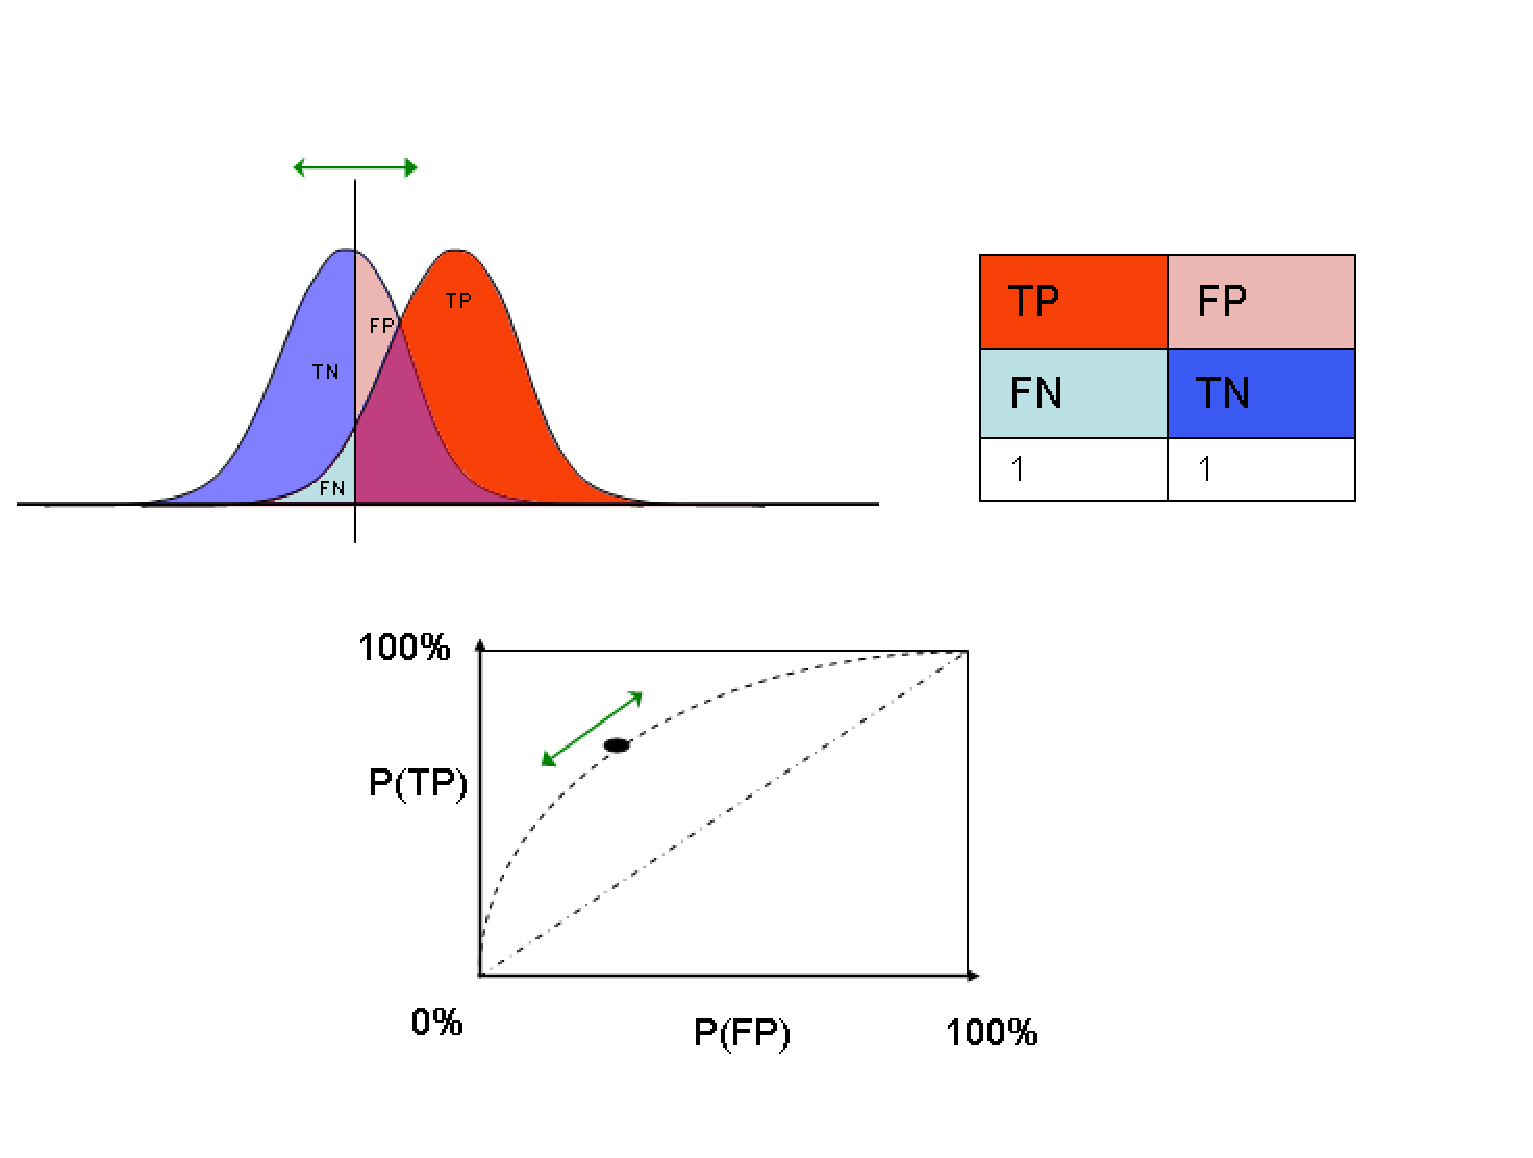
\includegraphics[height=0.75\textheight]{images/ROC_Class2Curve.eps}
		\caption{Perforamnce of a Classifier}
		\label{fig:ROCClass2Curve}
	\end{figure}
\end{frame}
%%%%%%%%%%%%%%%%%%%%%%%%%%%%%%%%%%%%%%%%%%%%%%%%%%%%%%%%%%%%%%%%%%%%%%%%%%%%%%%
\begin{frame}{ROC Curves III}
\begin{columns}[onlytextwidth]
\begin{column}{0.45\textwidth}
	\begin{figure}
		\centering
		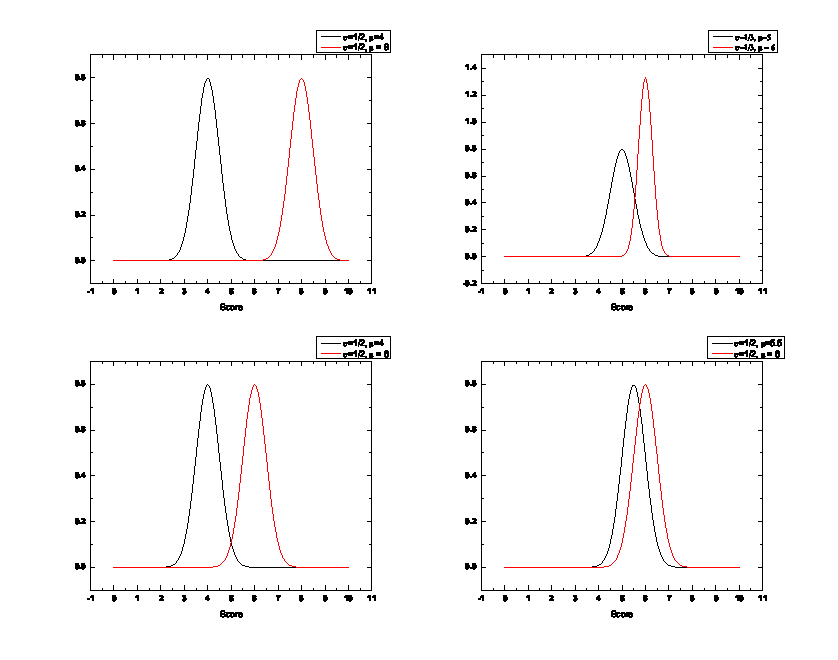
\includegraphics[height=\textwidth]{images/ROC_GaussDist.eps}
		\caption{Gaussian Classifers}
		\label{fig:ROCGausClassifers}
	\end{figure}
\end{column}
\begin{column}{0.45\textwidth}
	\begin{figure}
		\centering
		\includegraphics[height=\textwidth]{images/ROC_Gaussian.eps}
		\caption{ROC Curves of the Four Classifers}
		\label{fig:ROCGaussian}
	\end{figure}
\end{column}
\end{columns}
\end{frame}
%%%%%%%%%%%%%%%%%%%%%%%%%%%%%%%%%%%%%%%%%%%%%%%%%%%%%%%%%%%%%%%%%%%%%%%%%%%%%%%

% !TEX TS-program = pdflatex
% !TEX encoding = UTF-8 Unicode

% Matthew Urffer Master Thesis
% 
% Film Performance
%
\section{Film}

%%%%%%%%%%%%%%%%%%%%%%%%%%%%%%%%%%%%%%%%%%%%%%%%%%%%%%%%%%%%%%%%%%%%%%%%%%%%%%%
%                                                                             %
%                        FILM PERFORMANCE TABLES                              %
%                                                                             %
%%%%%%%%%%%%%%%%%%%%%%%%%%%%%%%%%%%%%%%%%%%%%%%%%%%%%%%%%%%%%%%%%%%%%%%%%%%%%%%
\subsection{Examples}
\begin{frame}{Example Spectra}
\begin{columns}[onlytextwidth]
\begin{column}{0.45\textwidth}
	\begin{figure}
		\centering
		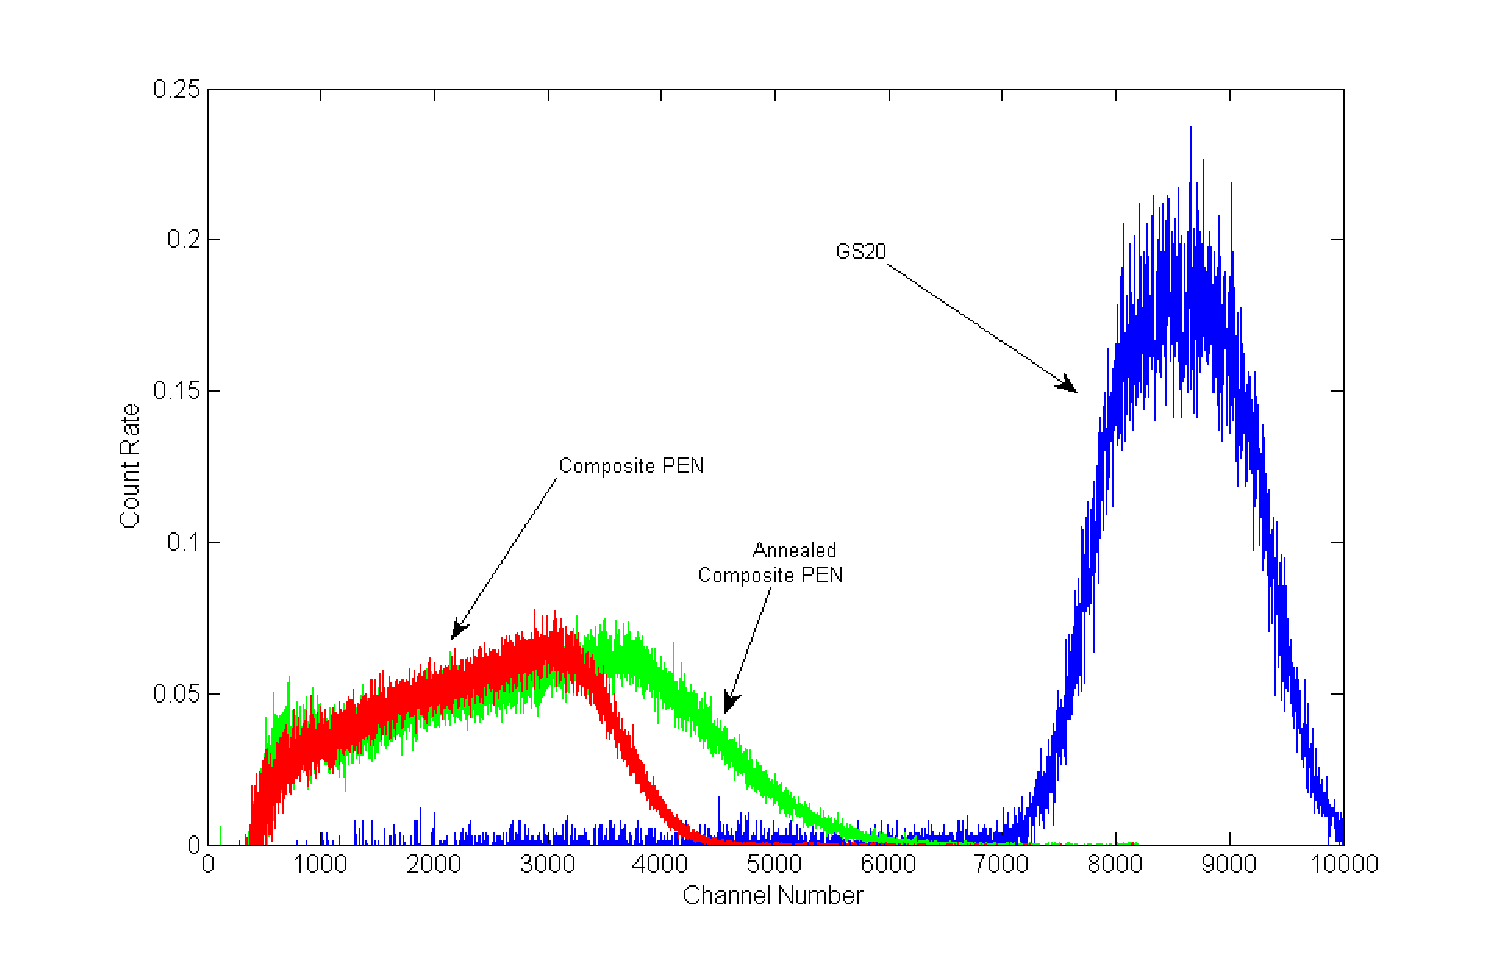
\includegraphics[width=\textwidth]{images/NeutronSpectra.eps}
		\caption{PEN Neutron Spectra}
		\label{fig:PENNeutronSpectra}
	\end{figure}
\end{column}
\begin{column}{0.45\textwidth}
	\begin{figure}
		\centering
		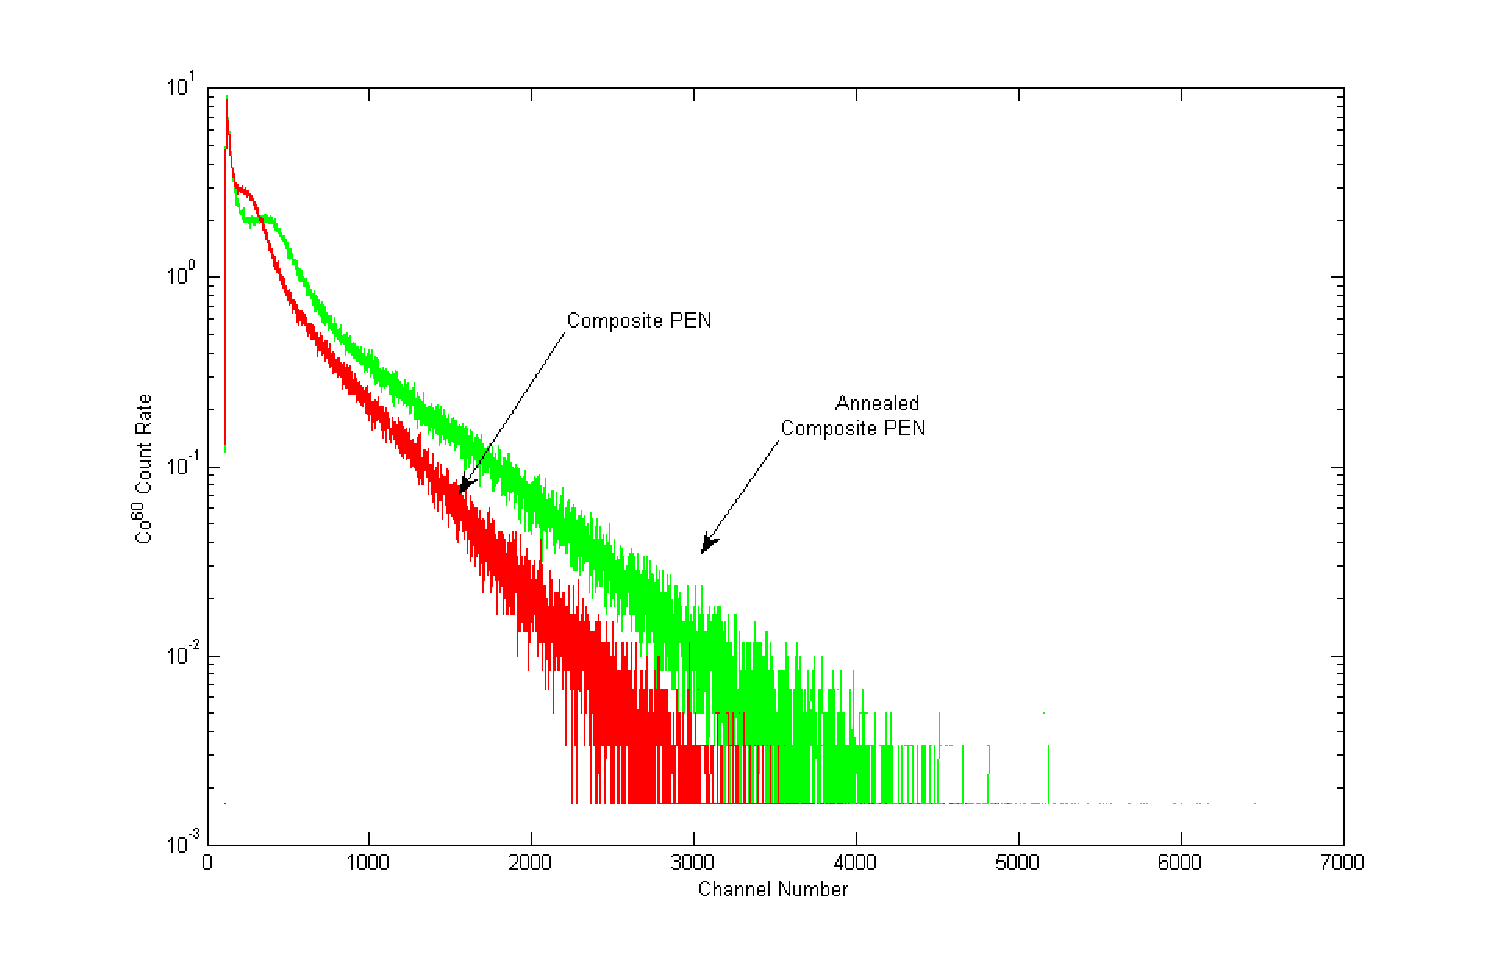
\includegraphics[width=\textwidth]{images/GammaSpectra.eps}
		\caption{PEN Gamma Spectra}
		\label{fig:PENGammaSpectra}
	\end{figure}
\end{column}
\end{columns}
\end{frame}

\subsection{Performance Tables}
%%%%%%%%%%%%%%%%%%%%%%%%%%%%%%%%%%%%%%%%%%%%%%%%%%%%%%%%%%%%%%%%%%%%%%%%%%%%%%%
\begin{frame}{Light Yield Performance}
	\begin{table}[h]
	\tiny
	\begin{tabular}{m{2cm} >{\centering\arraybackslash}m{1cm} >{\centering\arraybackslash}m{1cm} >{\centering\arraybackslash}m{1cm} >{\centering\arraybackslash}m{1cm} >{\centering\arraybackslash}m{1cm} >{\centering\arraybackslash}m{1cm}}
		 & Alpha Peak (${}^{241}$Am) & Beta Average (${}^{36}$Cl) & $\frac{\alpha}{<\beta>}$ & Photons per MeV (Gamma) & Photons per MeV (Beta) & Photons per MeV (Neutrons) \\
		 \hline
		 \hline
		 PEN 50 \% LiF 1\% ADS156FS (stretched) & 2,590 & 355 & 0.34 & 500 & 916 & 1,560 \\
		 \hdashline
		 PEN 70 \% LiF 25\% PPO/POPOPOP 5 \% (158 $\mu$m Annealed) &2,880 & 765 & 0.18 & 1,400 & 1,670 & 2,500 \\
		 \hdashline
		 PS  LiF 10\% PPO/POPOPOP 5 \% (26 $\mu$m Annealed) & 4,070 & 345 & 0.55 & 1,350 & 1,540 & 1,500\\
		 \hdashline
		 PS  LiF 30\% PPO/POPOPOP 5 \% (50 $\mu$m) & 3,490 & 393 & 0.41 & 1,140 & 1,120 & 1,120 \\
		 \hdashline
		 EJ-426 HD2 (LiF in ZnS:Ag) & & & & 19,750 &  & 26,900 \\
	\end{tabular}
	\end{table}
\end{frame}
%%%%%%%%%%%%%%%%%%%%%%%%%%%%%%%%%%%%%%%%%%%%%%%%%%%%%%%%%%%%%%%%%%%%%%%%%%%%%%%
\begin{frame}{Neutronic and Gamma Efficiency Performance}
	\begin{table}[h]
	\tiny
	\begin{tabular}{m{3cm} >{\centering\arraybackslash}m{2cm} >{\centering\arraybackslash}m{2cm} >{\centering\arraybackslash}m{2cm}}
		 & Absorber Mass (mg) & Total Neutron Count Rate (cps) & Neutron Count Rate above $\epsilon_{int,\gamma} \le 10^{-6}$ (cps) \\
		 \hline
		 \hline
		 PEN 50 \% LiF 1\% ADS156FS (stretched) & 9.10 & 53.04 & 11.45 \\
		 \hdashline
		 PEN 70 \% LiF 25\% PPO/POPOPOP 5 \% (158 $\mu$m Annealed) & 19.6 & 92.4 & 21.2 \\
		 \hdashline
		 PS  LiF 10\% PPO/POPOPOP 5 \% (26 $\mu$m Annealed) & 1.37 &8.25 & 2.25 \\
		 \hdashline
		 PS  LiF 30\% PPO/POPOPOP 5 \% (50 $\mu$m) & 9.33 & 82.64 & 1.01 \\
		 \hdashline
		 EJ-426 HD2 (LiF in ZnS:Ag) & 105 & 568.3 & 24.56 \\
	\end{tabular}
	\end{table}
\end{frame}



% !TEX TS-program = pdflatex
% !TEX encoding = UTF-8 Unicode

% Matthew Urffer Master Thesis
% 
% Sim Performance
%
\section{Simulation Results}

%%%%%%%%%%%%%%%%%%%%%%%%%%%%%%%%%%%%%%%%%%%%%%%%%%%%%%%%%%%%%%%%%%%%%%%%%%%%%%%
%                                                                             %
%                                 Single Film                                 %
%                                                                             %
%%%%%%%%%%%%%%%%%%%%%%%%%%%%%%%%%%%%%%%%%%%%%%%%%%%%%%%%%%%%%%%%%%%%%%%%%%%%%%%
\subsection*{Single Film}
%%%%%%%%%%%%%%%%%%%%%%%%%%%%%%%%%%%%%%%%%%%%%%%%%%%%%%%%%%%%%%%%%%%%%%%%%%%%%%%
\begin{frame}{Single Film Model}
\begin{columns}[onlytextwidth]
\begin{column}{0.45\textwidth}
\begin{itemize}
	\item Test configuration mocked up in MCNPX
	\item Single film simulated
\end{itemize}
	\tiny
	\begin{figure}
		\centering
		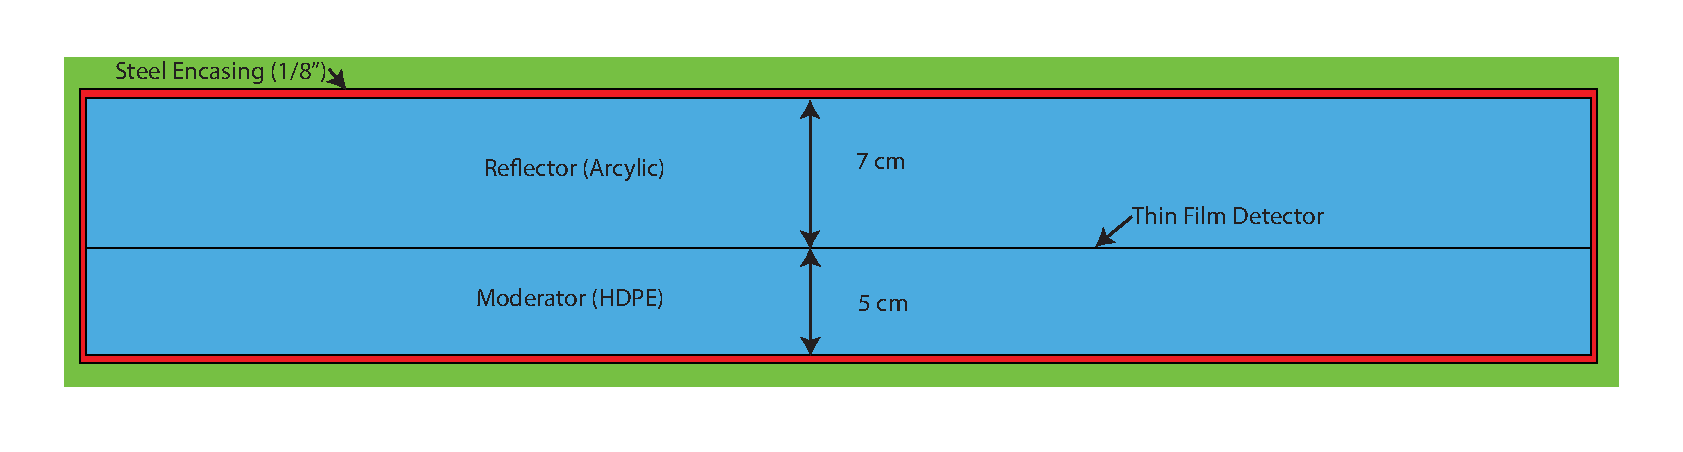
\includegraphics[width=\textwidth]{images/SingleFilm_DetectorAssembly.eps}
		\caption{Simulated RPM8 Detector}
	\end{figure}
\end{column}
\begin{column}{0.45\textwidth}
	\tiny
	\begin{figure}
		\centering
		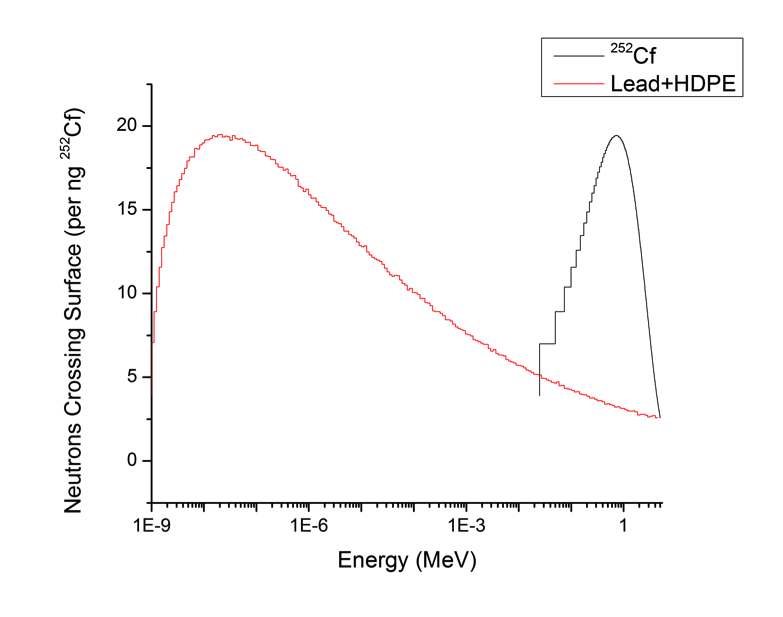
\includegraphics[width=\textwidth]{images/WattFission.eps}
		\caption{Source and incident Spectra}
	\end{figure}
\end{column}
\end{columns}
\end{frame}
%%%%%%%%%%%%%%%%%%%%%%%%%%%%%%%%%%%%%%%%%%%%%%%%%%%%%%%%%%%%%%%%%%%%%%%%%%%%%%%
\begin{frame}{Single layer optimization}
	\tiny
	\begin{itemize}
		\item Minimal optimization of the detector assembly was preformed
		\item Study on RPM8 encasing material
		\item Study on moderator and reflector thickness
		\item Count rate was too low
	\end{itemize}
	\begin{figure}
		\centering
		\includegraphics[height=0.55\textheight]{images/PS_50um_30LiF-InteractionRate-ShieldThickness.eps}
		\tiny \caption{Optimal Reflector and Moderator Study}
	\end{figure}
\end{frame}
%%%%%%%%%%%%%%%%%%%%%%%%%%%%%%%%%%%%%%%%%%%%%%%%%%%%%%%%%%%%%%%%%%%%%%%%%%%%%%%
%                                                                             %
%                                 Layered Films                               %
%                                                                             %
%%%%%%%%%%%%%%%%%%%%%%%%%%%%%%%%%%%%%%%%%%%%%%%%%%%%%%%%%%%%%%%%%%%%%%%%%%%%%%%
\subsection*{Layered Films}
%%%%%%%%%%%%%%%%%%%%%%%%%%%%%%%%%%%%%%%%%%%%%%%%%%%%%%%%%%%%%%%%%%%%%%%%%%%%%%%
\begin{frame}{Effects of Layering I}
\small
\begin{itemize}
	\item Single films are unable to have a high enough count rate
	\item Solution: Multiple films!
	\item Effects of layering multiple films tested with EJ-426HD2
\end{itemize}
\begin{columns}[onlytextwidth]
\begin{column}{0.45\textwidth}
	\tiny
	\begin{figure}
		\centering
		\includegraphics[height=0.6\textheight]{images/EJ426HD_LayeredDetector_MultiSheet.eps}
	\end{figure}
\end{column}
\begin{column}{0.45\textwidth}
	\tiny
	\begin{figure}
		\centering
		\includegraphics[width=\textwidth]{images/EJ426HD_LayeredDetector_SingleSheet.eps}
	\end{figure}
\end{column}
\end{columns}
\end{frame}
%%%%%%%%%%%%%%%%%%%%%%%%%%%%%%%%%%%%%%%%%%%%%%%%%%%%%%%%%%%%%%%%%%%%%%%%%%%%%%%
\begin{frame}{Effects of Layering II}
Observe an increased neutron count rate \dots
	\begin{figure}
		\centering
		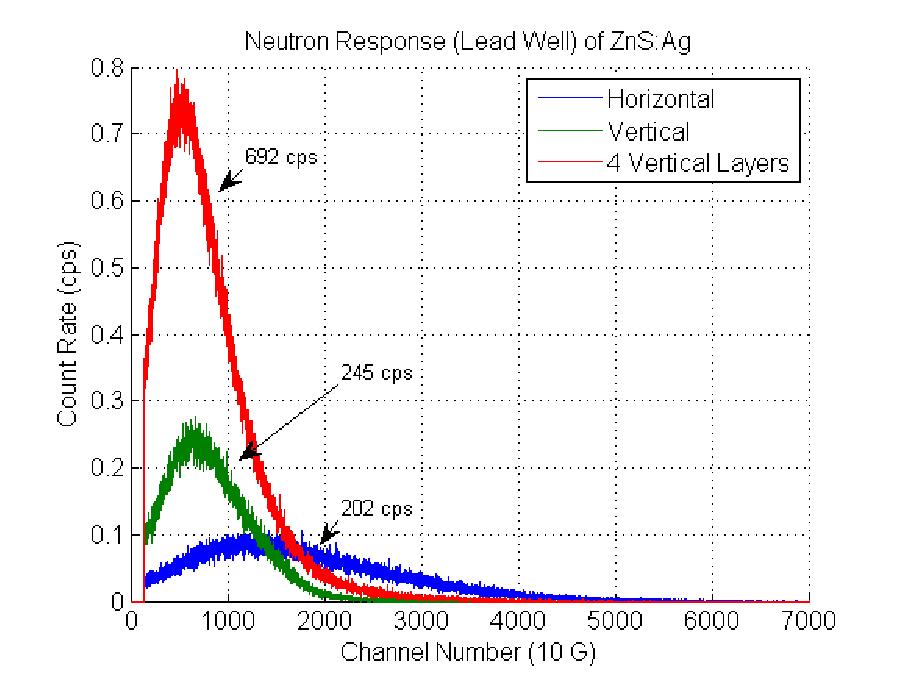
\includegraphics[height=0.6\textheight]{images/EJ426HD_Multi_NeutronComparison.eps}
		\small \caption{Neutron Spectra of EJ426HD2}
	\end{figure}
\end{frame}
%%%%%%%%%%%%%%%%%%%%%%%%%%%%%%%%%%%%%%%%%%%%%%%%%%%%%%%%%%%%%%%%%%%%%%%%%%%%%%%
\begin{frame}{Effects of Layering III}
with only a minimal increase in the gamma response!
\begin{columns}[onlytextwidth]
\begin{column}{0.45\textwidth}
	\tiny
	\begin{figure}
		\centering
		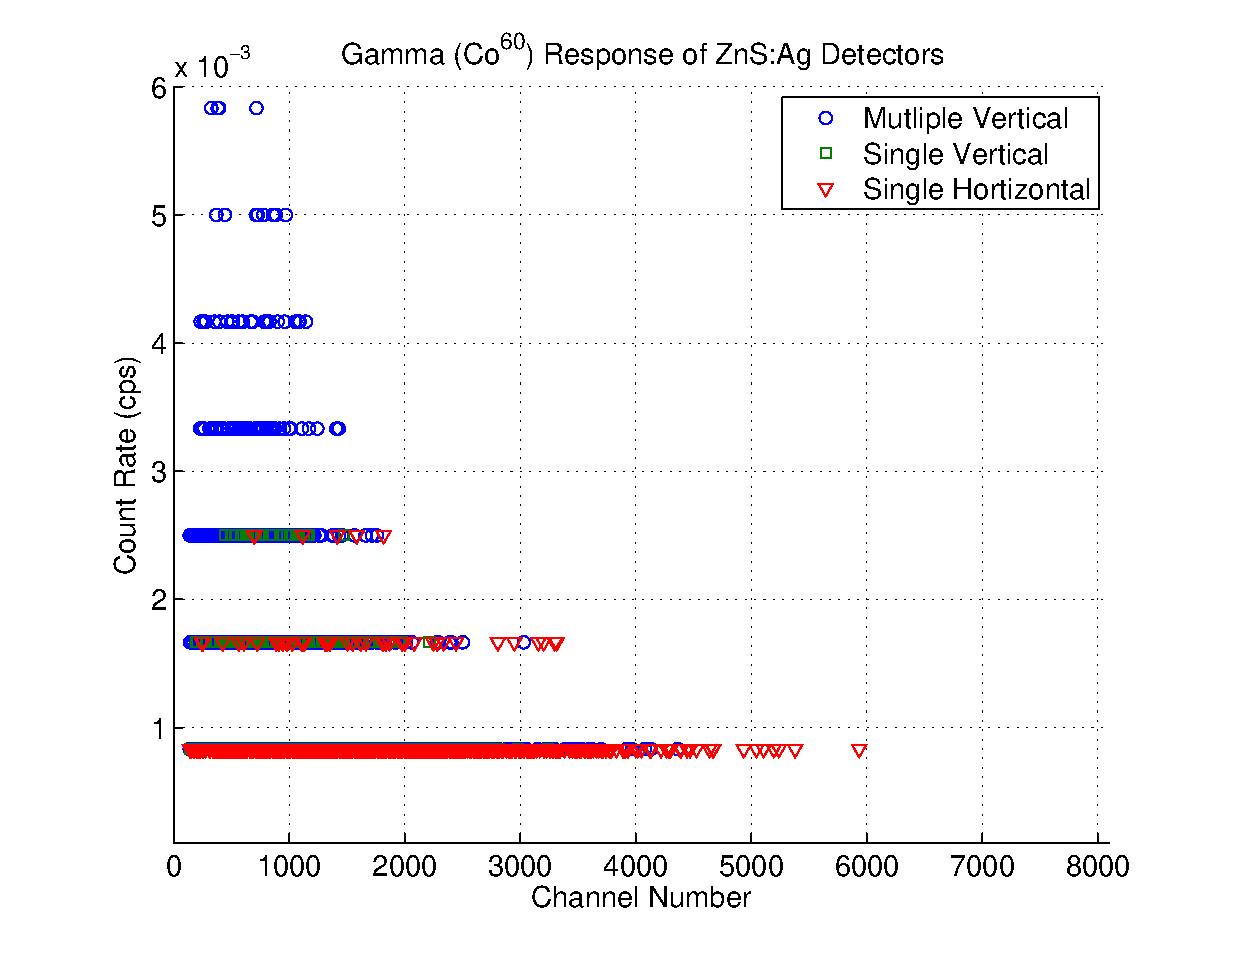
\includegraphics[width=\textwidth]{images/EJ426HD_Multi_GammaComparison.eps}
		\caption{Gamma Spectra of EJ426HD2}
	\end{figure}
\end{column}
\begin{column}{0.45\textwidth}
	\tiny
	\begin{figure}
		\centering
		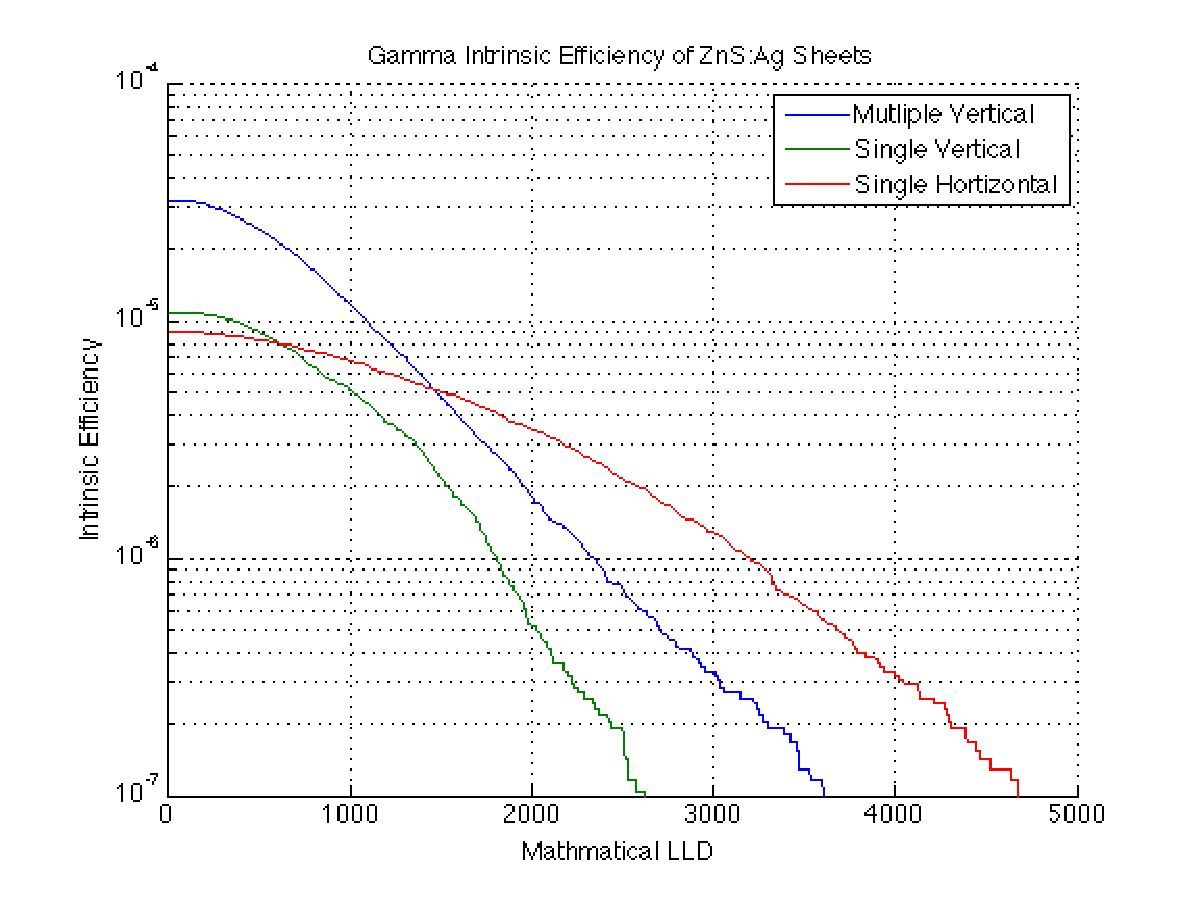
\includegraphics[width=\textwidth]{images/EJ426HD_Multi_GammaIntEff.eps}
		\caption{Gamma Intrinsic Efficiency of EJ426-HD2}
\end{figure}
\end{column}
\end{columns}
\end{frame}
%%%%%%%%%%%%%%%%%%%%%%%%%%%%%%%%%%%%%%%%%%%%%%%%%%%%%%%%%%%%%%%%%%%%%%%%%%%%%%%
\begin{frame}{Multi Film Model}
\begin{columns}[onlytextwidth]
\begin{column}{0.45\textwidth}
\small
120 50$\mu$m PS Films simulated
	\tiny
	\begin{figure}
		\centering
		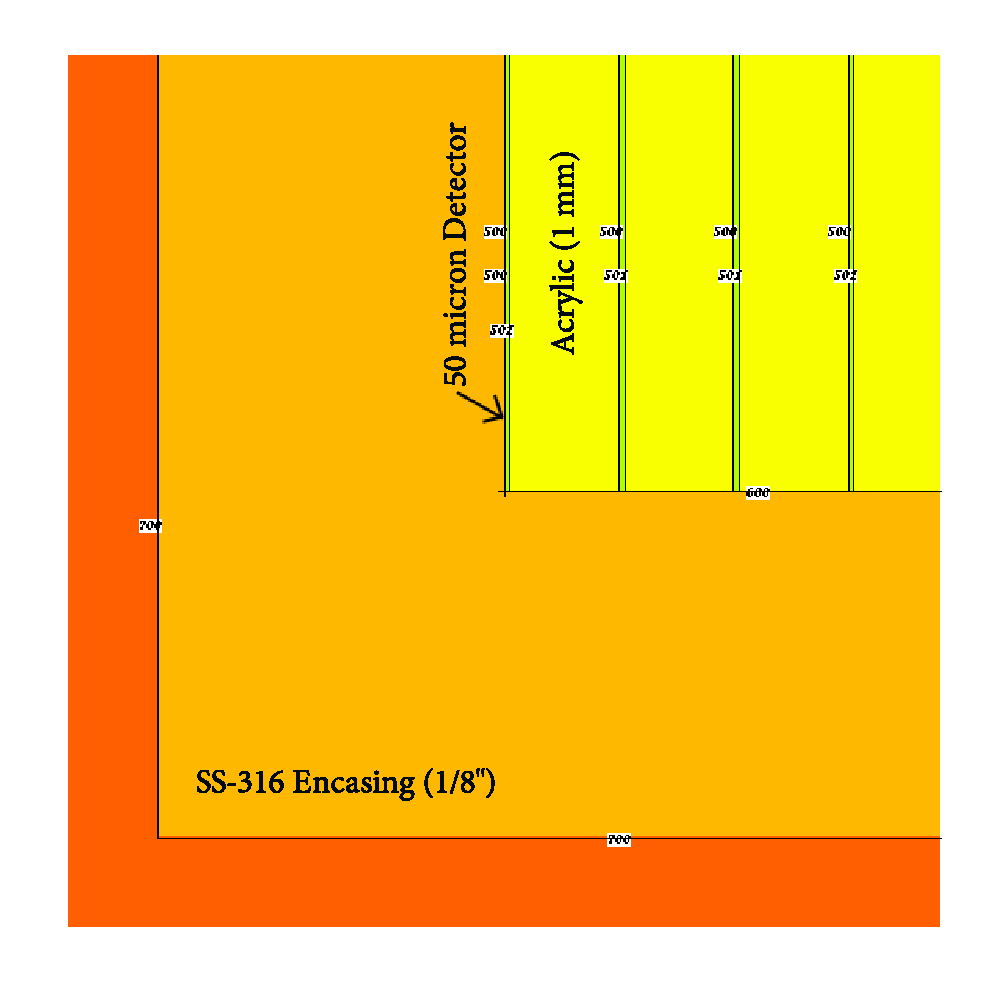
\includegraphics[width=\textwidth]{images/Multi_120Layers.eps}
		\caption{Simulated RPM8 Detector (120 layers)}
	\end{figure}
\end{column}
\begin{column}{0.45\textwidth}
	\tiny
	\begin{figure}
		\centering
		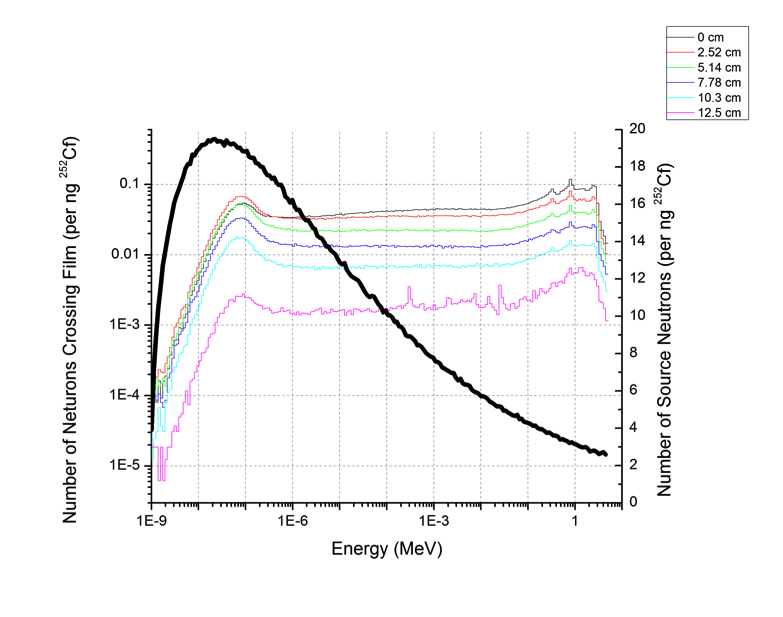
\includegraphics[width=\textwidth]{images/Spectra_Layered.eps}
		\caption{Source and Incident Spectra}
	\end{figure}
\end{column}
\end{columns}
\end{frame}
%%%%%%%%%%%%%%%%%%%%%%%%%%%%%%%%%%%%%%%%%%%%%%%%%%%%%%%%%%%%%%%%%%%%%%%%%%%%%%%
\begin{frame}{Minimum Number of Films}
	\small
	Minimum number of films needed was calculated
	\tiny
	\begin{itemize}
		\item 38 for LiF ZnS:Ag
		\item 74 for PEN
		\item 110 for PS
	\end{itemize}
	\tiny
	\begin{figure}
		\centering
		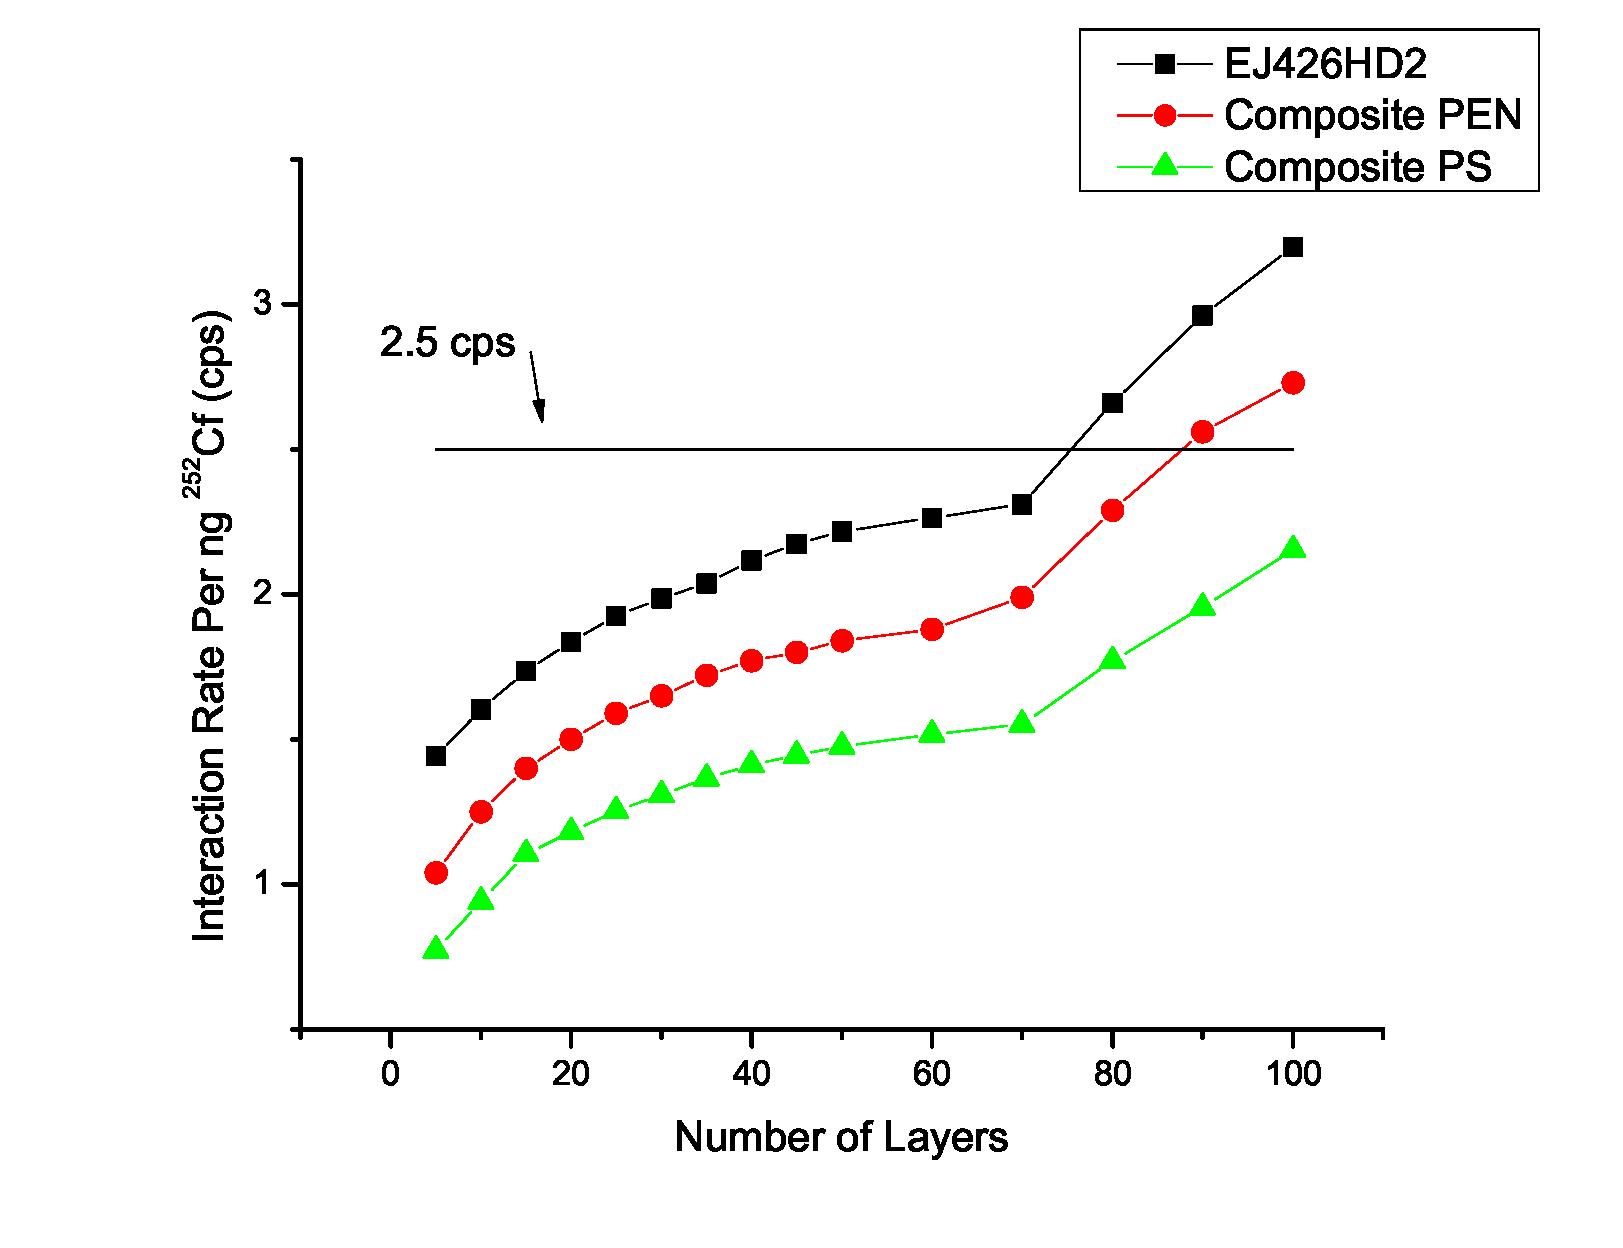
\includegraphics[height=0.6\textheight]{images/OptimalDetectorSize.eps}
		\tiny \caption{Minimum Required Layers}
	\end{figure}
\end{frame}
%%%%%%%%%%%%%%%%%%%%%%%%%%%%%%%%%%%%%%%%%%%%%%%%%%%%%%%%%%%%%%%%%%%%%%%%%%%%%%%

% !TEX TS-program = pdflatex
% !TEX encoding = UTF-8 Unicode

% Matthew Urffer Master Thesis
% 
% PSD Performance
%
\section{PSD Performance}

%%%%%%%%%%%%%%%%%%%%%%%%%%%%%%%%%%%%%%%%%%%%%%%%%%%%%%%%%%%%%%%%%%%%%%%%%%%%%%%
%                                                                             %
%                               PSD PERFORMANCE                               %
%                                                                             %
%%%%%%%%%%%%%%%%%%%%%%%%%%%%%%%%%%%%%%%%%%%%%%%%%%%%%%%%%%%%%%%%%%%%%%%%%%%%%%%
\subsection*{PS Films}
%%%%%%%%%%%%%%%%%%%%%%%%%%%%%%%%%%%%%%%%%%%%%%%%%%%%%%%%%%%%%%%%%%%%%%%%%%%%%%%
\begin{frame}{PSD Performance (PS Films I)}
\small
\begin{itemize}
	\item Enhanced performance can be achieved with PSD (theoretically)
	\item PS films show some ability for PSD
	\item None of the films are optimized \cite{zaitseva_plastic_2012}
\end{itemize}
\begin{columns}[onlytextwidth]
\begin{column}{0.30\textwidth}
	\tiny
	\begin{figure}
		\centering
		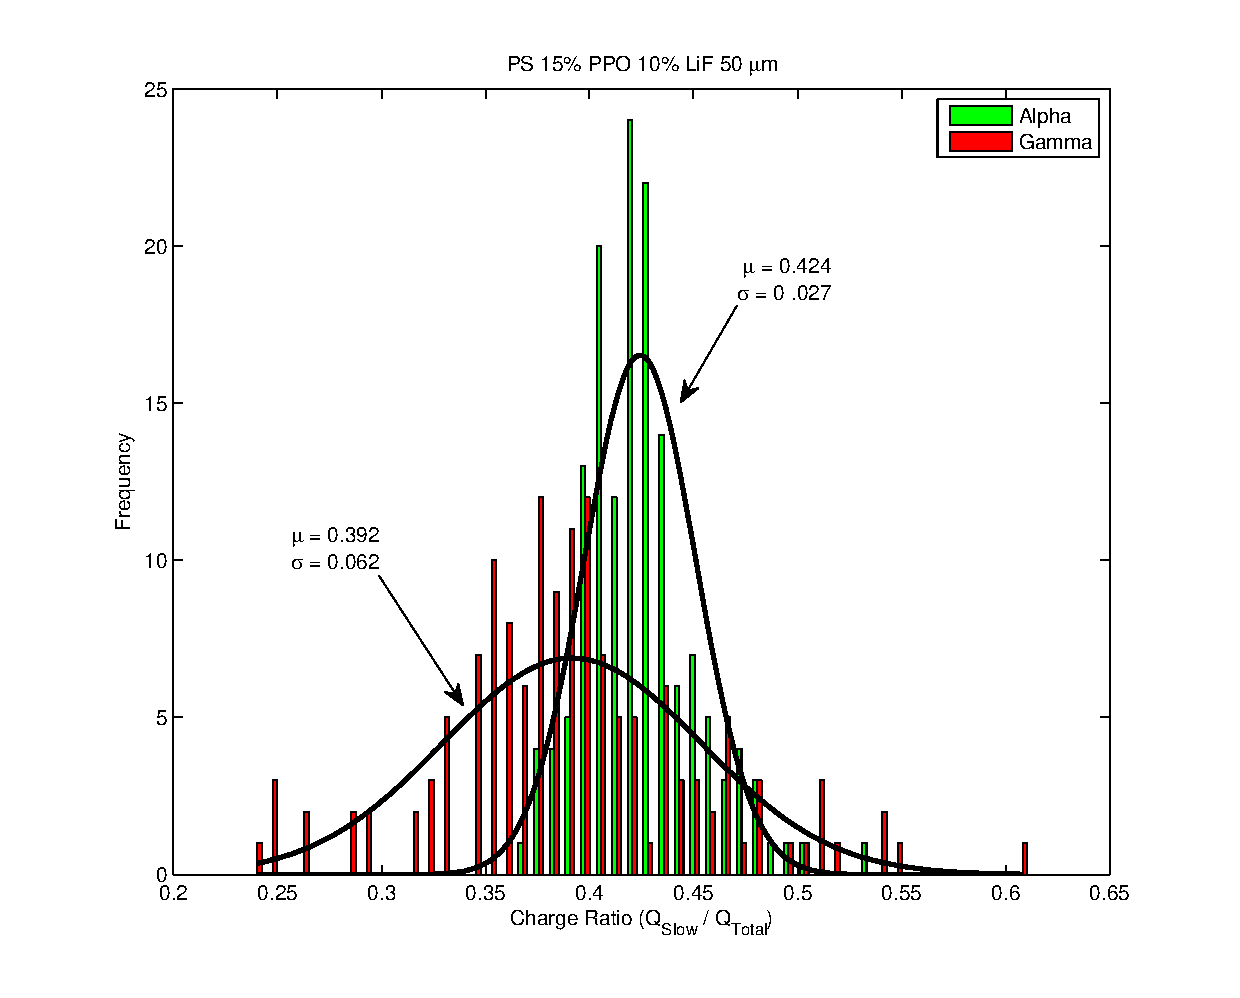
\includegraphics[width=\textwidth]{images/ChargeIntegration_PS_LiF_POP_50um.eps}
		\caption{PS 10\% LiF 50 $\mu$m}
	\end{figure}
\end{column}
\begin{column}{0.30\textwidth}
	\tiny
	\begin{figure}
		\centering
		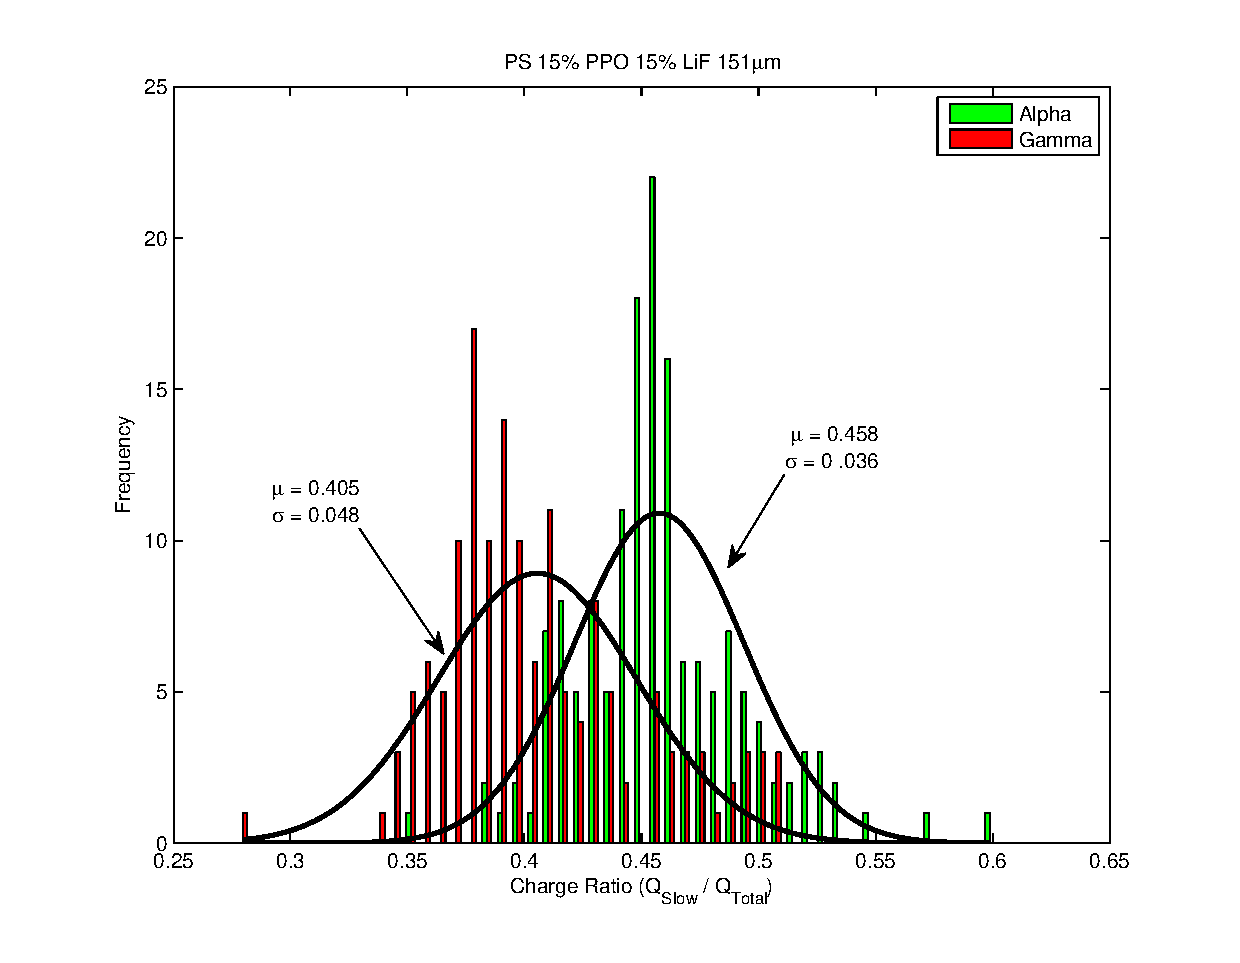
\includegraphics[width=\textwidth]{images/ChargeIntegration_PS_LiF_POP_151um.eps}
		\caption{PS 10\% LiF 150 $\mu$m}
	\end{figure}
\end{column}
\begin{column}{0.30\textwidth}
	\tiny
	\begin{figure}
		\centering
		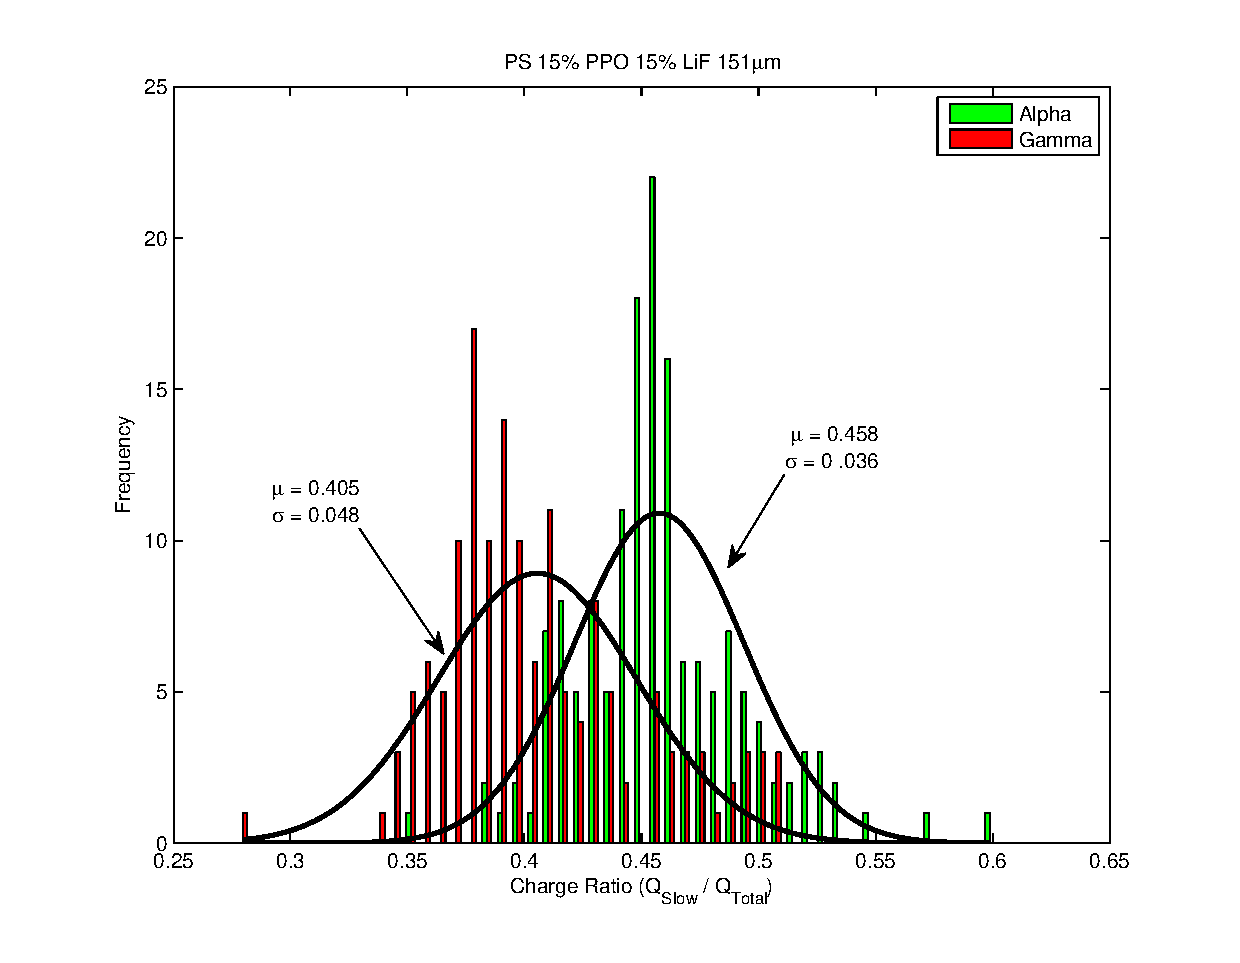
\includegraphics[width=\textwidth]{images/ChargeIntegration_PS_LiF15_POP_151um.eps}
		\caption{PS 15\% LiF 150 $\mu$m}
	\end{figure}
\end{column}
\end{columns}
\end{frame}
%%%%%%%%%%%%%%%%%%%%%%%%%%%%%%%%%%%%%%%%%%%%%%%%%%%%%%%%%%%%%%%%%%%%%%%%%%%%%%%
\begin{frame}{PSD Performance (PS Films II)}
\small
\begin{itemize}
	\item Thicker films tend to have better PSD
	\item Additional LiF decrease PSD performance
\end{itemize}
\begin{columns}[onlytextwidth]
\begin{column}{0.45\textwidth}
	\tiny
	\begin{figure}
		\centering
		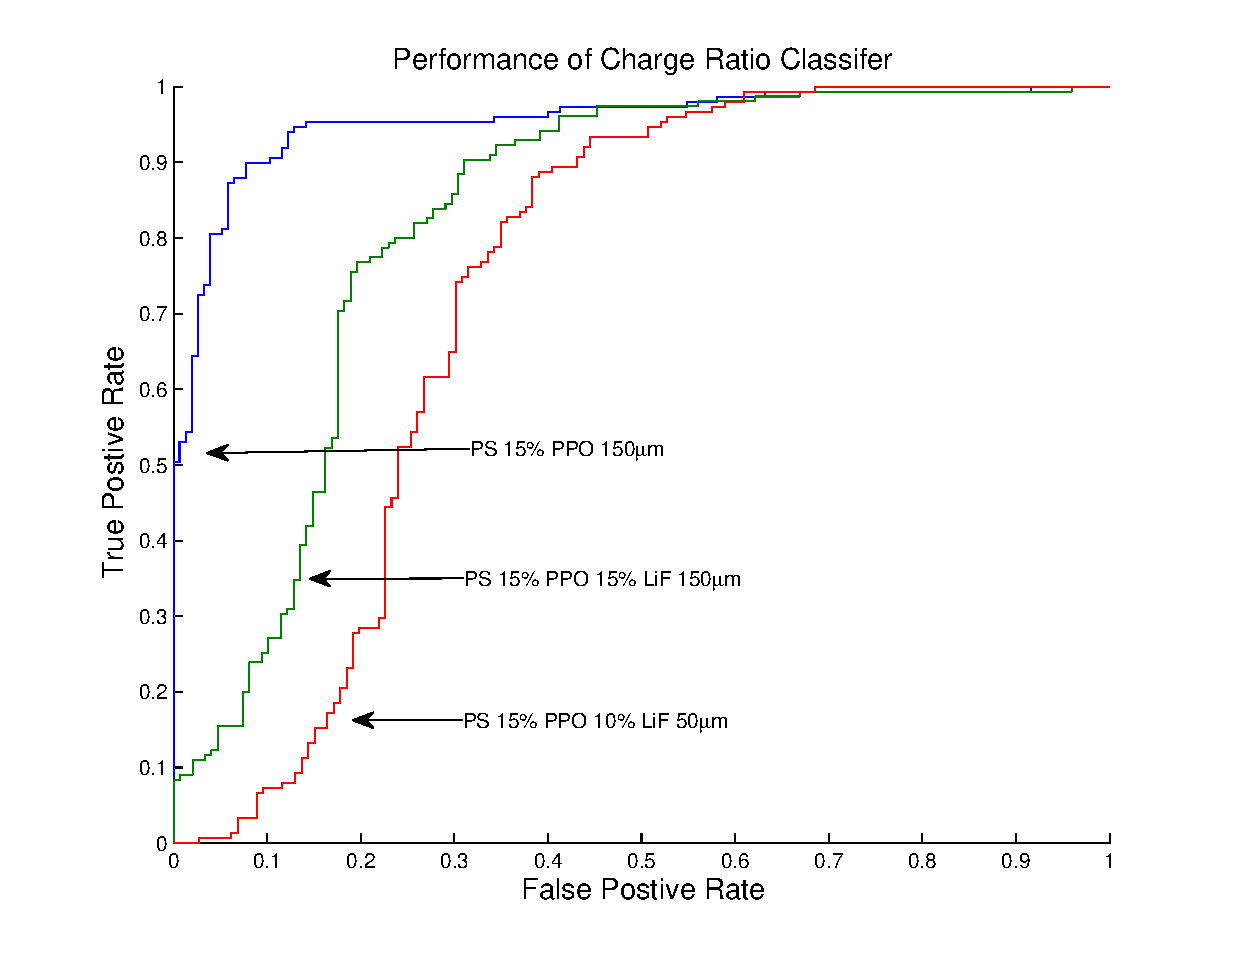
\includegraphics[width=\textwidth]{images/ROC_Comparison.eps}
		\caption{ROC Curves of Charge Integration Classifier (PS Films)}
	\end{figure}
\end{column}
\begin{column}{0.45\textwidth}
	\tiny
	\begin{figure}
		\centering
		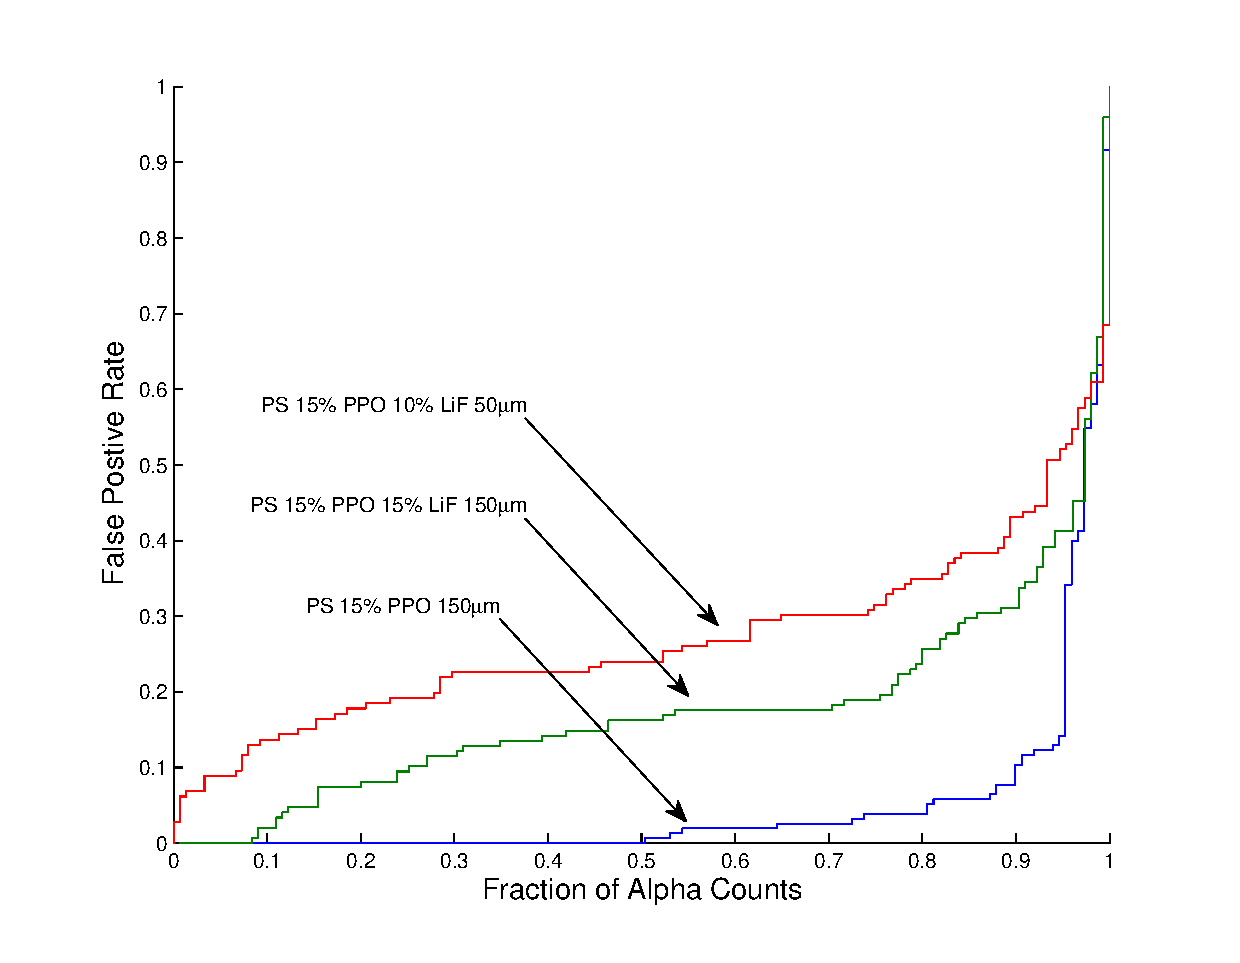
\includegraphics[width=\textwidth]{images/FPRvsFractionCounts_Comparison.eps}
		\caption{Possible Configuration}
	\end{figure}
\end{column}
\end{columns}
\end{frame}
%%%%%%%%%%%%%%%%%%%%%%%%%%%%%%%%%%%%%%%%%%%%%%%%%%%%%%%%%%%%%%%%%%%%%%%%%%%%%%%
\subsection*{PEN Films}
%%%%%%%%%%%%%%%%%%%%%%%%%%%%%%%%%%%%%%%%%%%%%%%%%%%%%%%%%%%%%%%%%%%%%%%%%%%%%%%
\begin{frame}{PSD Performance (PEN Films)}
\small
\begin{itemize}
	\item PEN films demonstrated little capability for PSD
	\item PEN films where mounted on Katpon, which scintillates
	\item None of the films are optimized \cite{zaitseva_plastic_2012}
\end{itemize}
	\begin{figure}
		\centering
		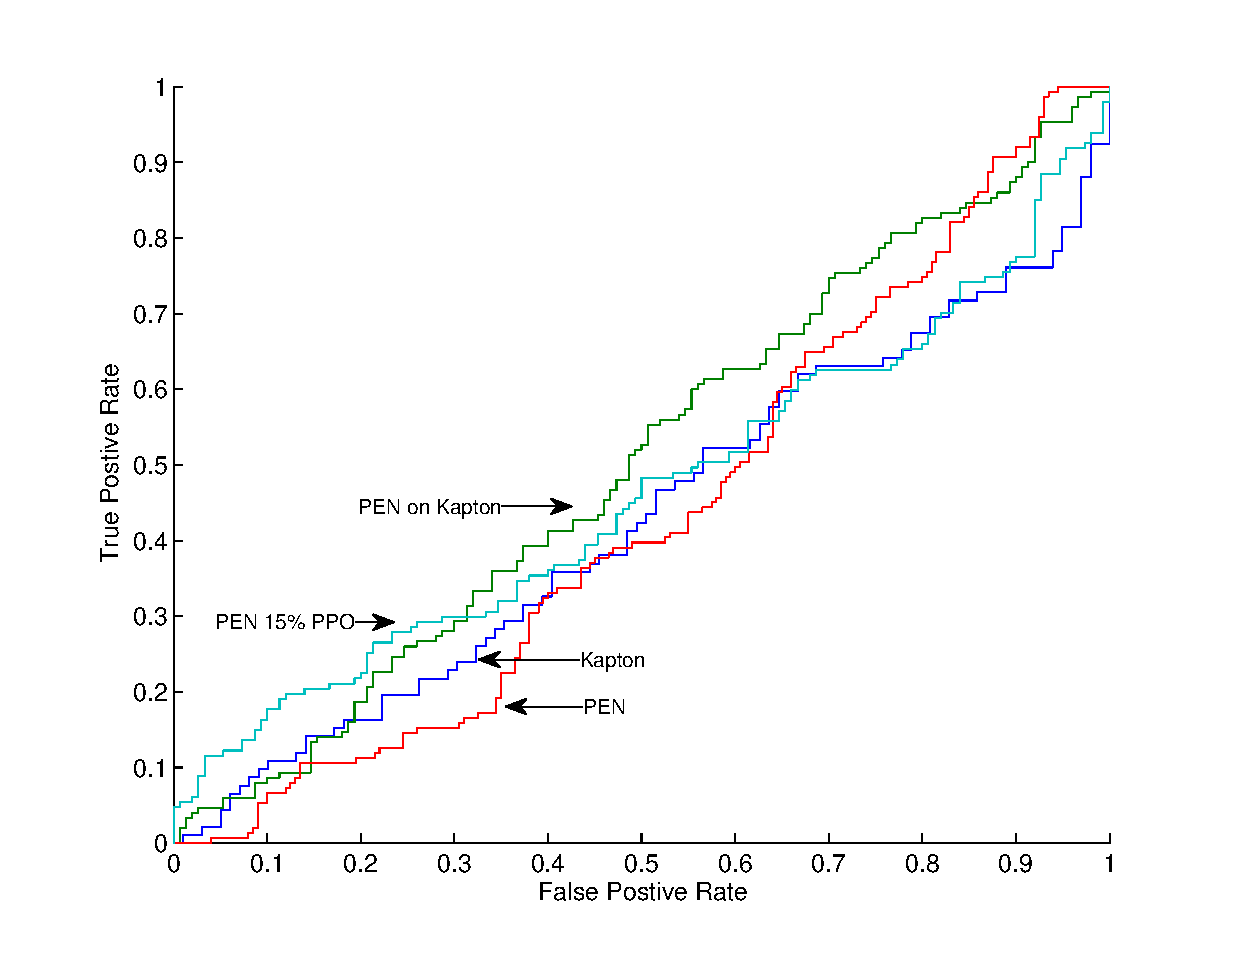
\includegraphics[height=0.55\textheight]{images/PEN_ROC_Comparison.eps}
		\caption{ROC Curves of Charge Integration Classifier (PEN Films)}
	\end{figure}
\end{frame}

\section*{Summary}

\begin{frame}{Summary}

  \begin{itemize}
  \item
    A framework has been developed for the characterization of possible replacement technologies for radiation portal monitors
  \item
    A framework has been developed for pulse shape discrimination 
  \item
    Thin polymeric films have been demonstrated to have the necessary interaction rates for radiation portal monitors
  \end{itemize}
 \large
 Questions?
\end{frame}


% BILBIOLGRAPHY
\begin{frame}[allowframebreaks]
\frametitle{Works Cited}
	\tiny
    \bibliography{Zotero}
\end{frame}

% APPENDIX
\appendix
\section<presentation>*{\appendixname}
\subsection<presentation>*{Fundamental Physics}
\begin{frame}{Absorption Cross Sections}
\begin{figure}
	\centering
		\includegraphics[width=0.9\textwidth]{images/CrossSections.eps}
	\caption{Cross sections of selected isotopes \protect \cite{nist_neutron_2012}}
	\label{fig:CrossSections}
\end{figure}

\end{frame}




\end{document}


